\documentclass[11pt]{article}
\usepackage{fullpage}
\usepackage{setspace}
\usepackage{amsmath}
\usepackage{fancyvrb}
\usepackage{enumerate}
\usepackage{pgfplots}
\usepackage{graphicx}
\usepackage{float}
%\usepackage{multirow}
\usepackage[format=hang,labelsep=quad]{caption}
\usepackage{subfig}
\usepackage{array}
\usepackage{multirow}
%\usepackage{subcaption}

\renewcommand\thesubfigure{\roman{subfigure}}


\begin{document}
\noindent\large{Math 5365}\\
\large{Data Mining 1}\\
\large{Homework 8}\\
\large{Mary Barker}
\doublespace
\begin{enumerate}
\item For the following problems, consult the HouseVotes84 data set.
  \begin{enumerate}
    \item What is the probability that a randomly selected representative is a Democrat? 

    The probability is roughly 61\%. 
    \item Given that a representative is a Republican, what is the probability that he or 
          she voted for water project cost sharing? 

          The probability is apprimately 38.5 \%. 
    \item Given that a representative voted for adoption of the budget resolution, 
          against the physician fee freeze and duty free exports, find the probabilty that 
          he or she is a Democrat (Hint: if x is a vector, you can use \verb|rbind(x)| to 
          force R to treat it as a row vector. You can set missing values of x to NA and 
          naive Bayes will ignore them.)

         The conditional probability that the representative will be a Democrat is approximately 
         86.4 \%
  \end{enumerate}

\item Investigate the normality of the quantitative variables in the wdbc.data data set, using 
Shapiro-Wilk tests, histograms, and qq-plots. 

The $p-$values for each of the variables using the Shapiro-Wilkes test are shown below. 

From a brief inspection, it can be seen that all of the values are extremely small. The larges value is 
approximately 0.0002. 
Thus it can be argued that none of the quantitative variables in the wdbc.data set are 
normally distributed. 

\begin{center}
\begin{tabular}{|cc | cc|}
\hline
V3  &  3.10564350835627e-14 &  V18 &  1.08295733912683e-23 \\ 
V4  &  7.2835810327422e-08  &  V19 &  1.10168126780958e-31 \\
V5  &  7.01140152099188e-15 &  V20 &  7.82599801678132e-17 \\
V6  &  3.19626432303972e-22 &  V21 &  3.12680667408936e-24 \\
V7  &  8.60083255698697e-05 &  V22 &  8.55101761746864e-31 \\
V8  &  3.96720386388631e-17 &  V23 &  1.7042937076837e-17 \\
V9  &  1.33857097282064e-21 &  V24 &  2.56446728764913e-06 \\
V10 &  1.4045559983538e-19  &  V25 &  1.37333569710147e-17 \\
V11 &  7.8847728112006e-09  &  V26 &  5.5953643813558e-25 \\
V12 &  1.95657476081236e-16 &  V27 &  0.000209699323707618 \\
V13 &  1.22459720865597e-28 &  V28 &  1.24746121547919e-19 \\
V14 &  3.56060098095499e-19 &  V29 &  4.54330018415444e-17 \\
V15 &  7.5874879541832e-30  &  V30 &  1.98487847266396e-10 \\
V16 &  2.65270327436955e-35 &  V31 &  3.23378464163622e-17 \\
V17 &  1.36196704959636e-23 &  V32 &  9.1951455450728e-20 
\tabularnewline
\hline
\end{tabular}
\end{center}

Since the Shapiro-Wilk test is highly sensitive and can give small $p-$values for close-to-normally 
distributed data, another method for investigating the data is to view the distribution in plot form.  

For each of the columns in wdbc, the histogram and qq norm plots are shown. 

\begin{figure}[H]
\begin{center}
\subfloat[]{\begin{centering}
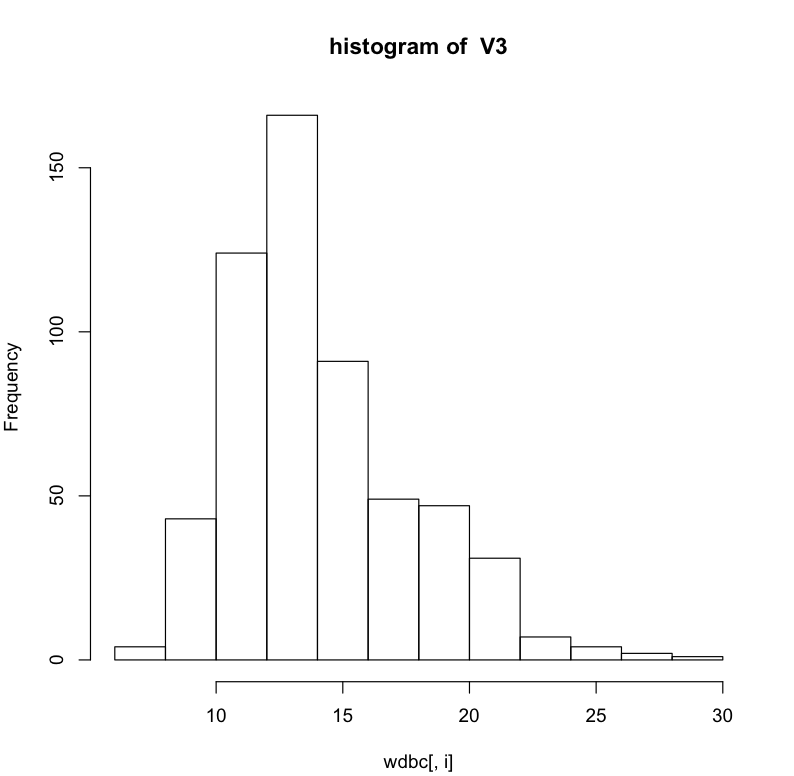
\includegraphics[scale=0.225]{pix/h_v3}
\par\end{centering}}
\quad{}
\subfloat[]{\begin{centering}
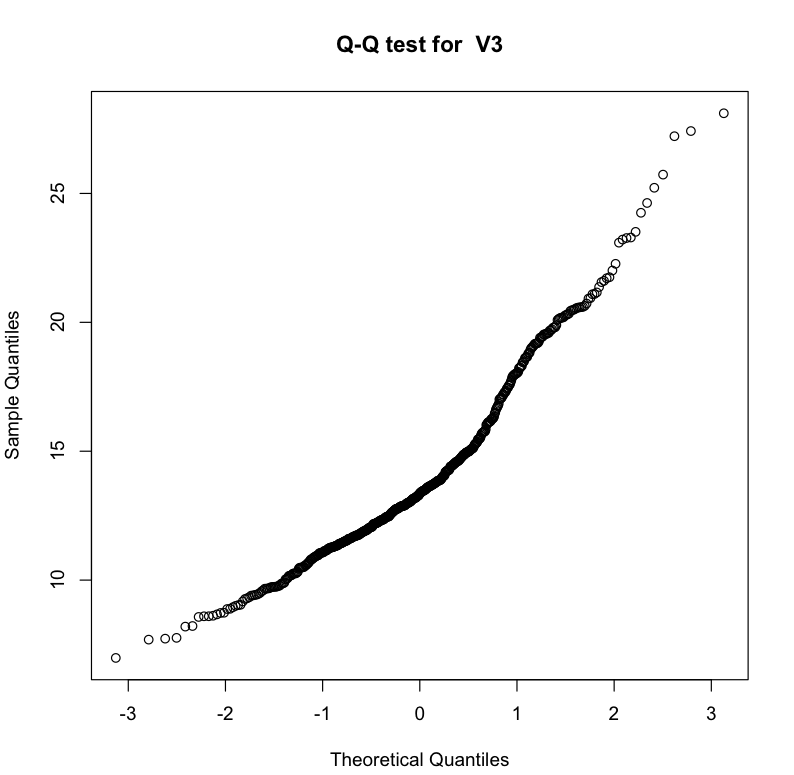
\includegraphics[scale=0.225]{pix/q_v3}
\par\end{centering}}
\quad{}
\subfloat[]{\begin{centering}
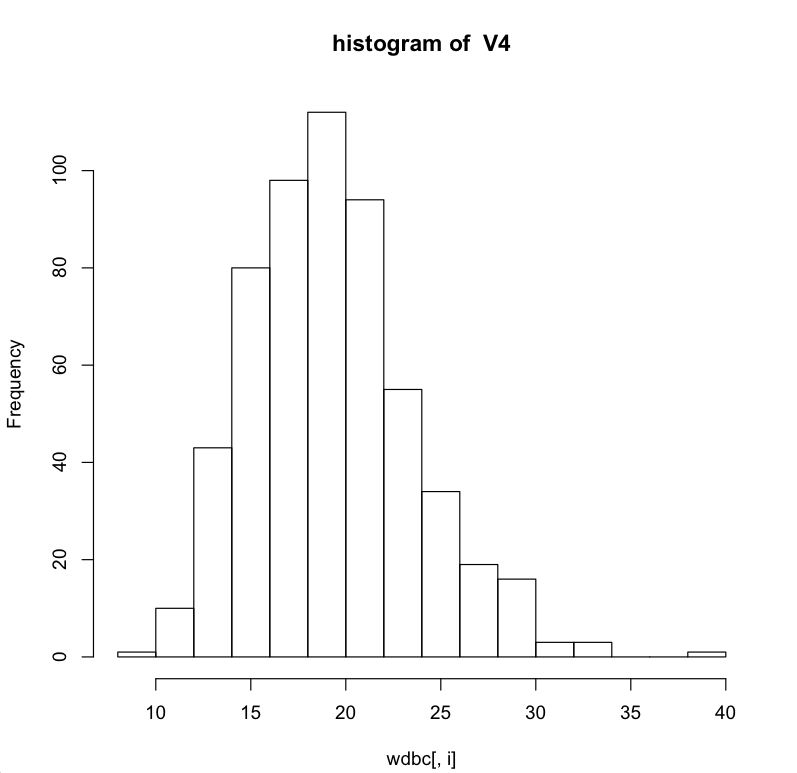
\includegraphics[scale=0.225]{pix/h_v4}
\par\end{centering}}
\quad{}
\subfloat[]{\begin{centering}
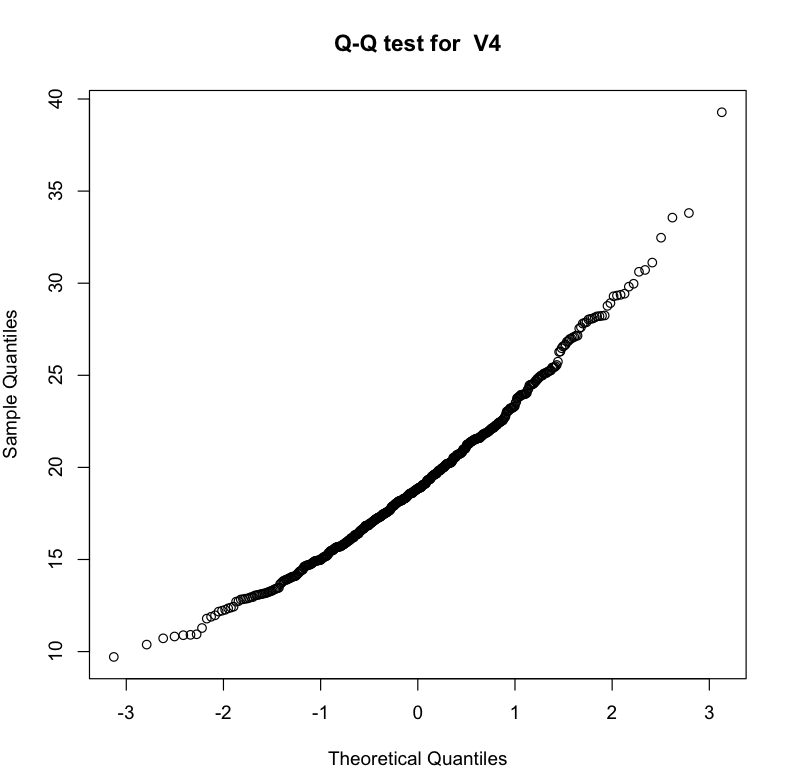
\includegraphics[scale=0.225]{pix/q_v4}
\par\end{centering}}
\quad{}
\subfloat[]{\begin{centering}
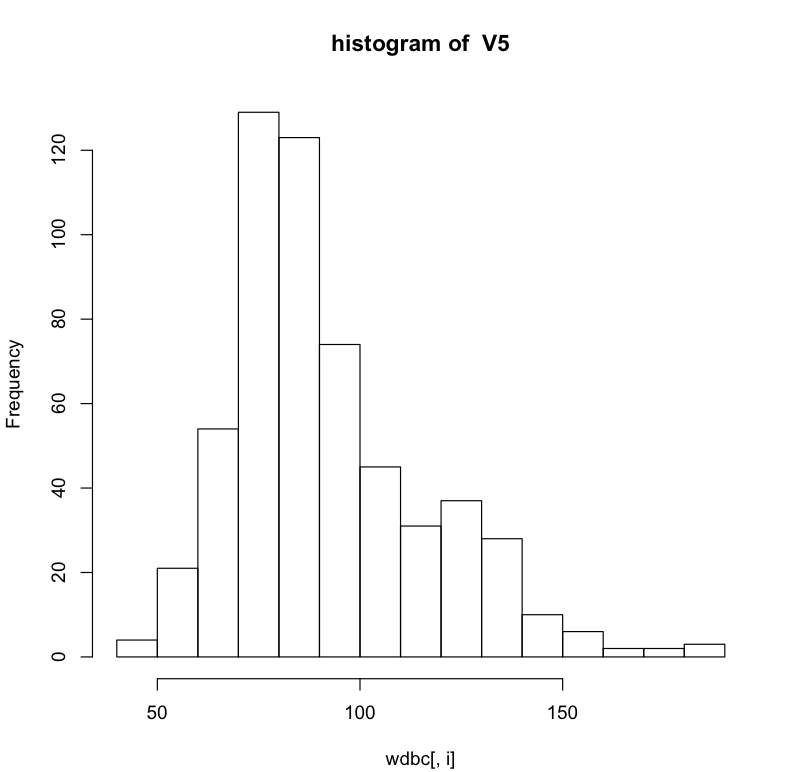
\includegraphics[scale=0.225]{pix/h_v5}
\par\end{centering}}
\quad{}
\subfloat[]{\begin{centering}
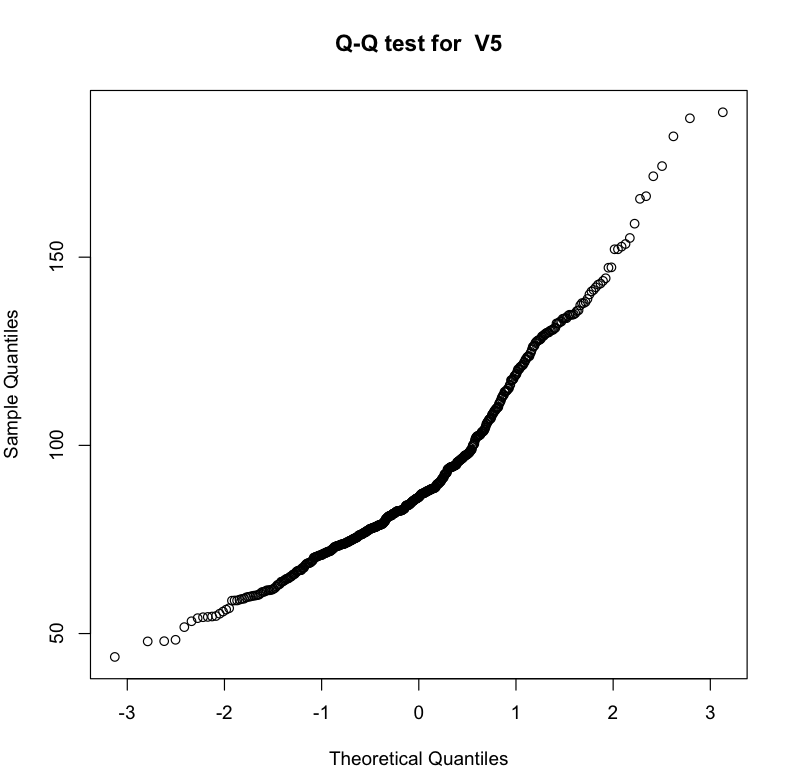
\includegraphics[scale=0.225]{pix/q_v5}
\par\end{centering}}
\end{center}
\end{figure}

\begin{figure}[H]
\begin{center}
\subfloat[]{\begin{centering}
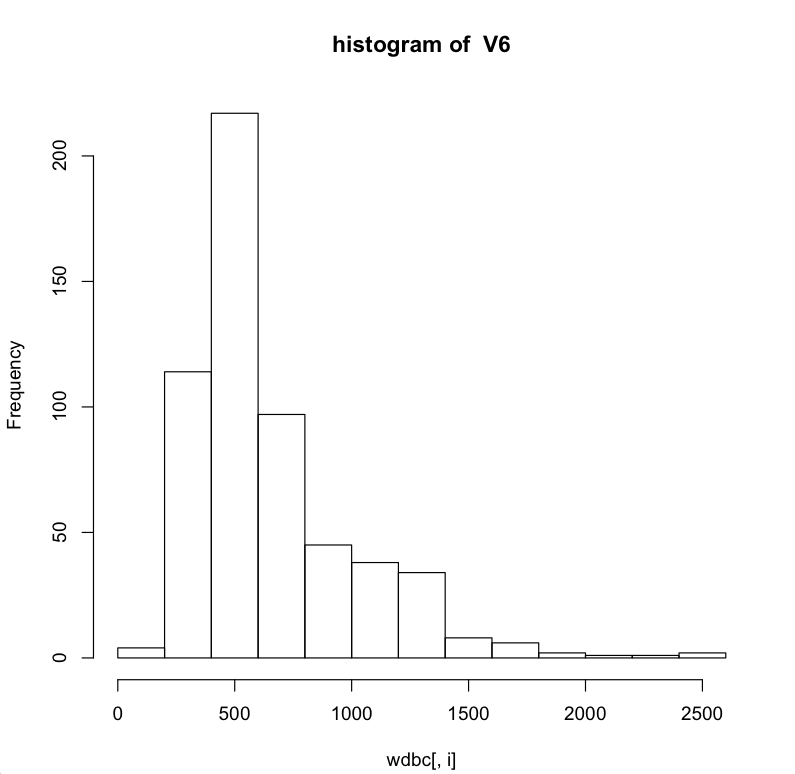
\includegraphics[scale=0.225]{pix/h_v6}
\par\end{centering}}
\quad{}
\subfloat[]{\begin{centering}
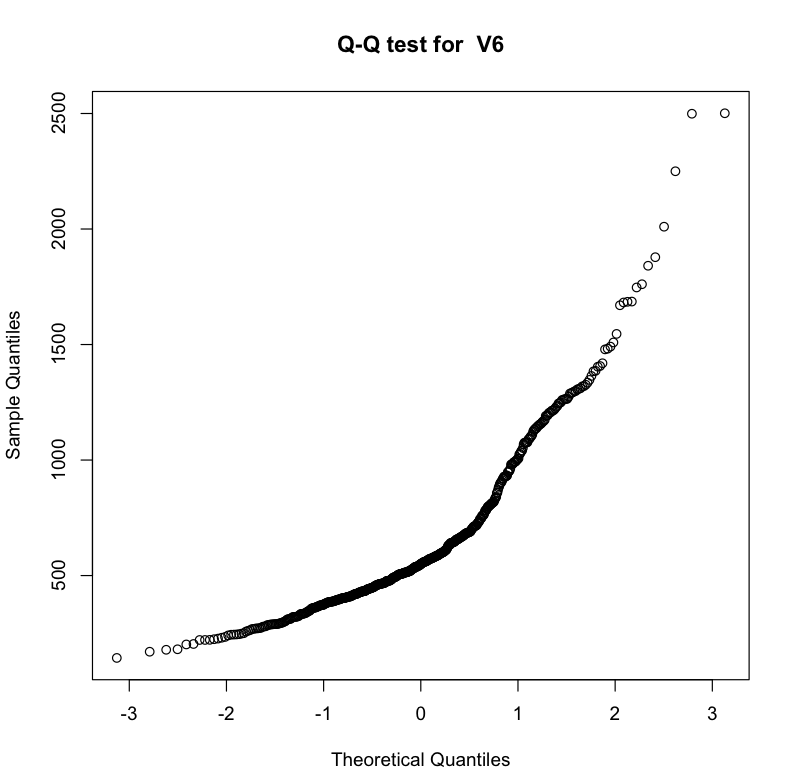
\includegraphics[scale=0.225]{pix/q_v6}
\par\end{centering}}
\quad{}
\subfloat[]{\begin{centering}
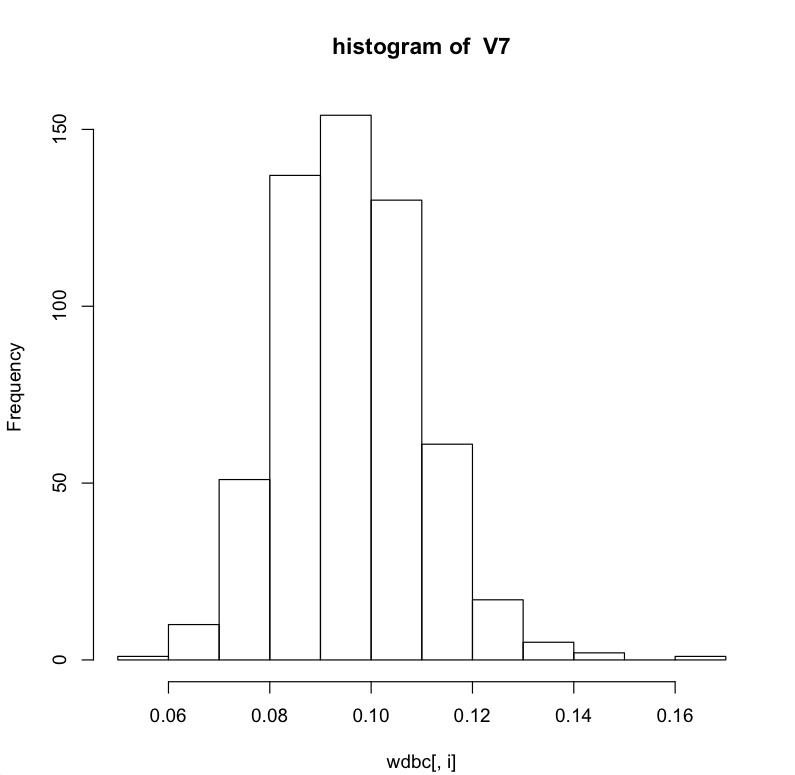
\includegraphics[scale=0.225]{pix/h_v7}
\par\end{centering}}
\quad{}
\subfloat[]{\begin{centering}
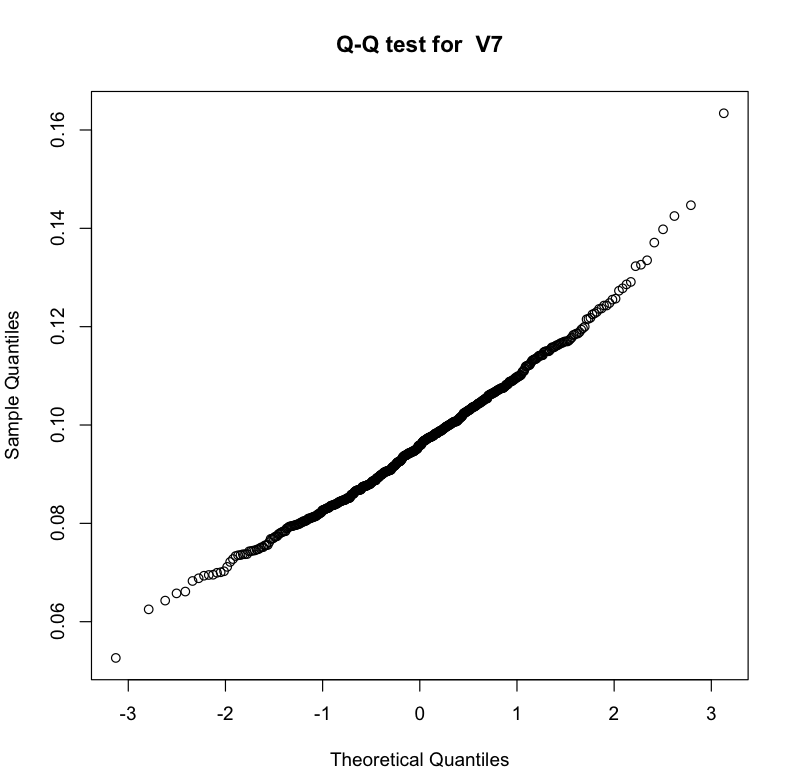
\includegraphics[scale=0.225]{pix/q_v7}
\par\end{centering}}
\quad{}
\subfloat[]{\begin{centering}
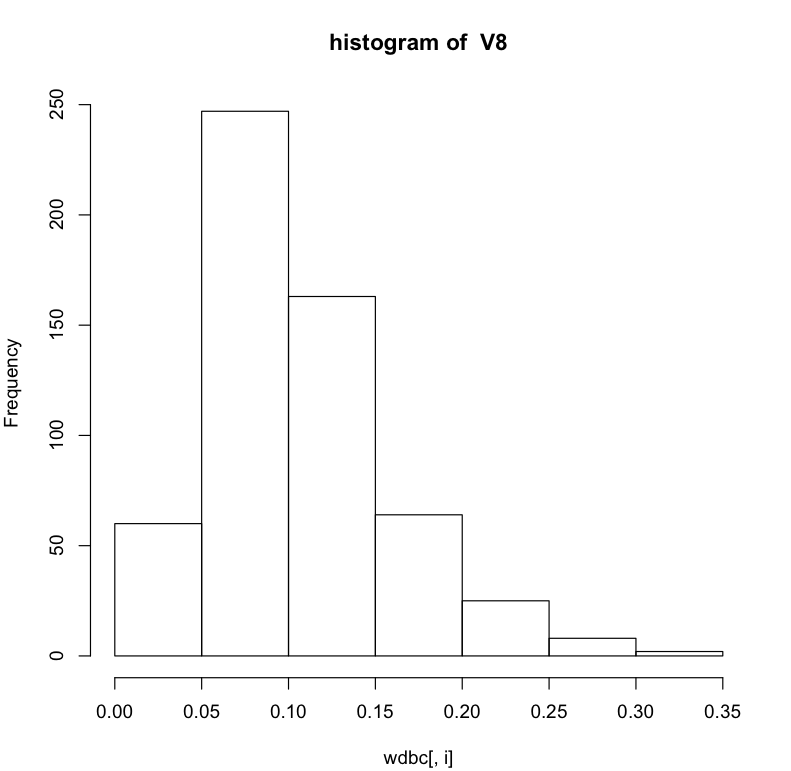
\includegraphics[scale=0.225]{pix/h_v8}
\par\end{centering}}
\quad{}
\subfloat[]{\begin{centering}
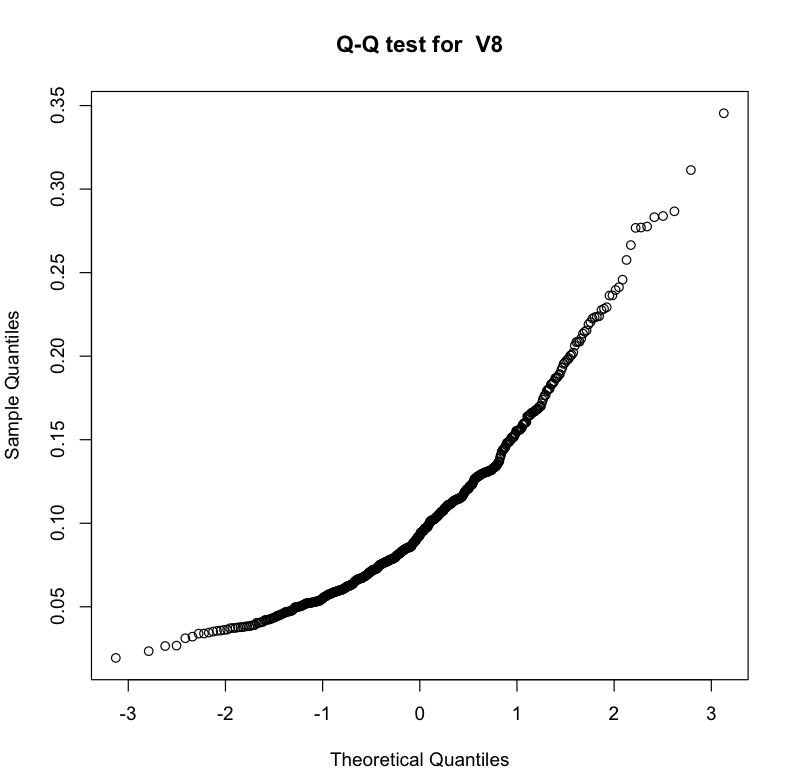
\includegraphics[scale=0.225]{pix/q_v8}
\par\end{centering}}
\end{center}
\end{figure}

\begin{figure}[H]
\begin{center}
\subfloat[]{\begin{centering}
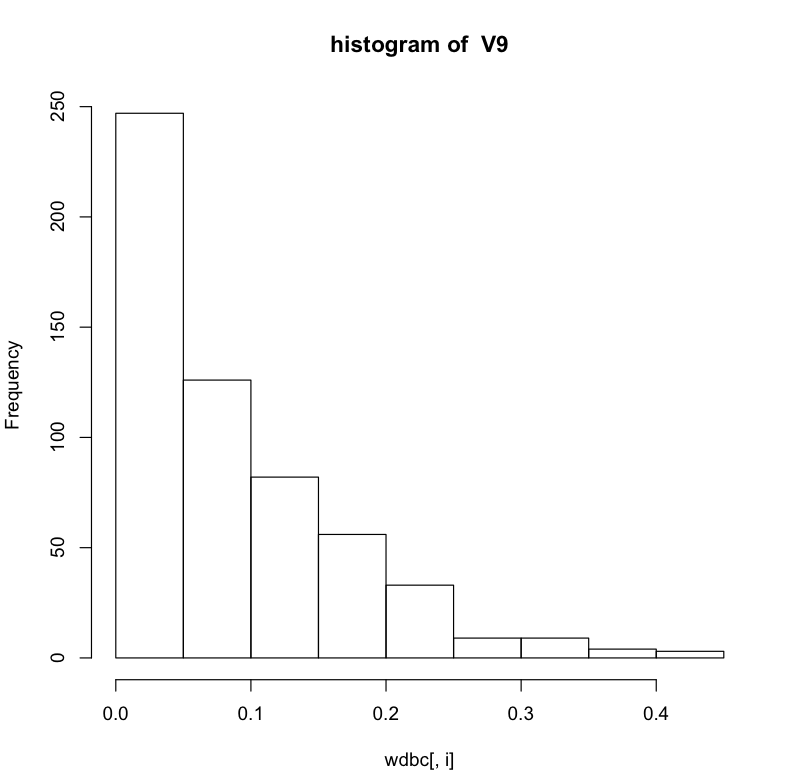
\includegraphics[scale=0.225]{pix/h_v9}
\par\end{centering}}
\quad{}
\subfloat[]{\begin{centering}
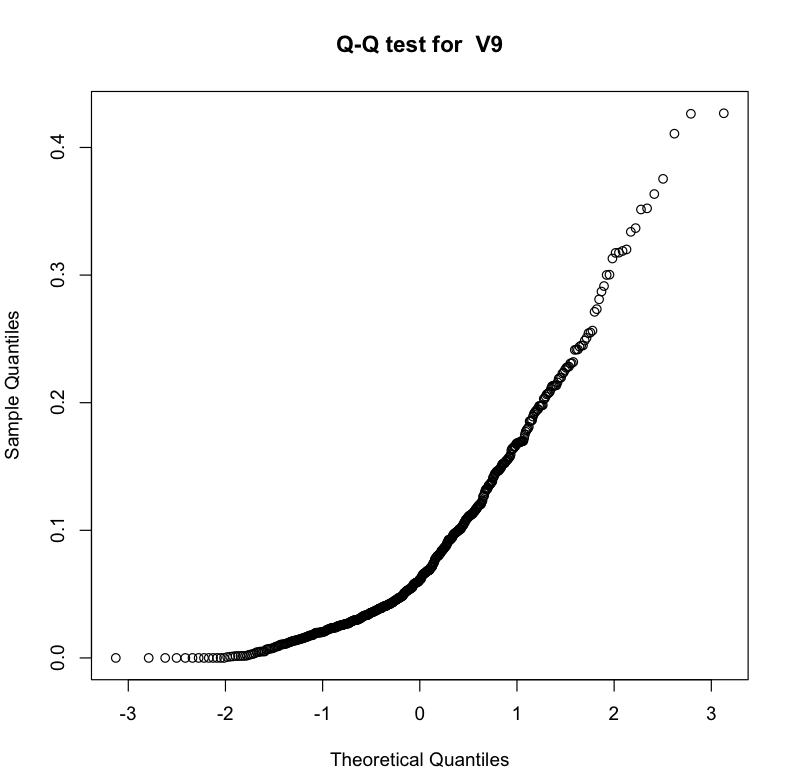
\includegraphics[scale=0.225]{pix/q_v9}
\par\end{centering}}
\quad{}
\subfloat[]{\begin{centering}
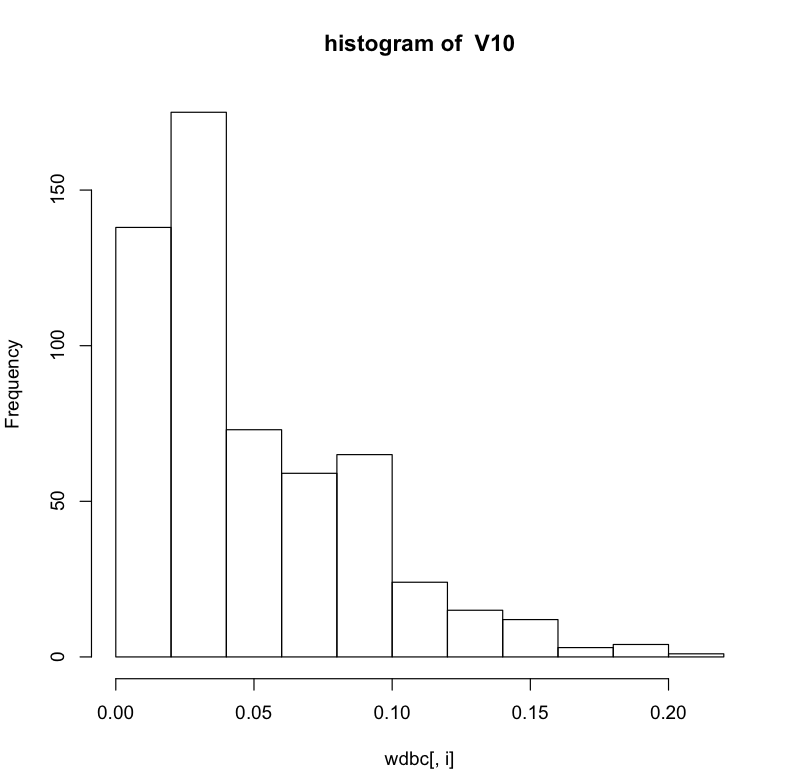
\includegraphics[scale=0.225]{pix/h_v10}
\par\end{centering}}
\quad{}
\subfloat[]{\begin{centering}
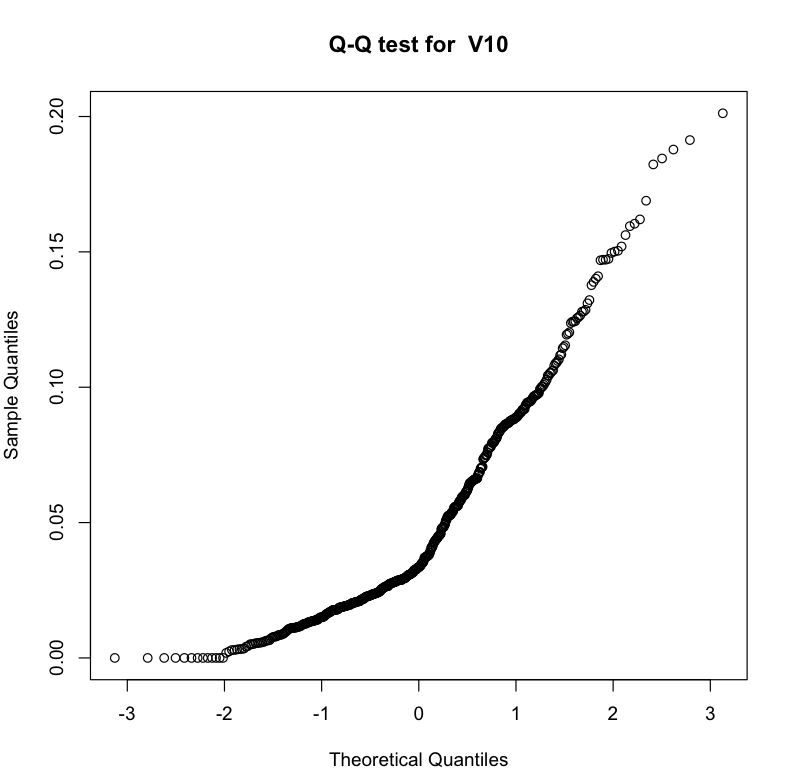
\includegraphics[scale=0.225]{pix/q_v10}
\par\end{centering}}
\quad{}
\subfloat[]{\begin{centering}
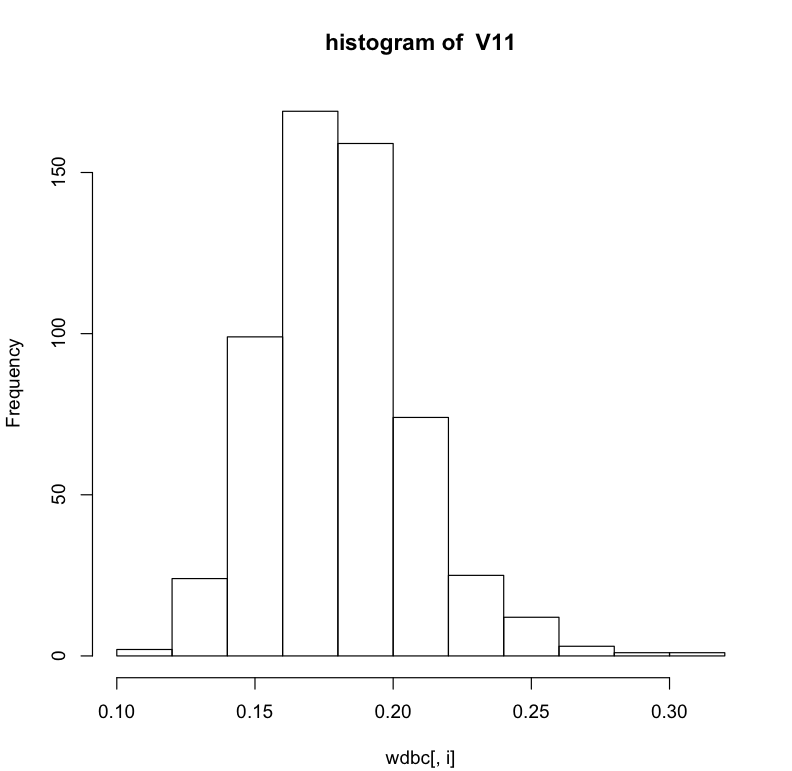
\includegraphics[scale=0.225]{pix/h_v11}
\par\end{centering}}
\quad{}
\subfloat[]{\begin{centering}
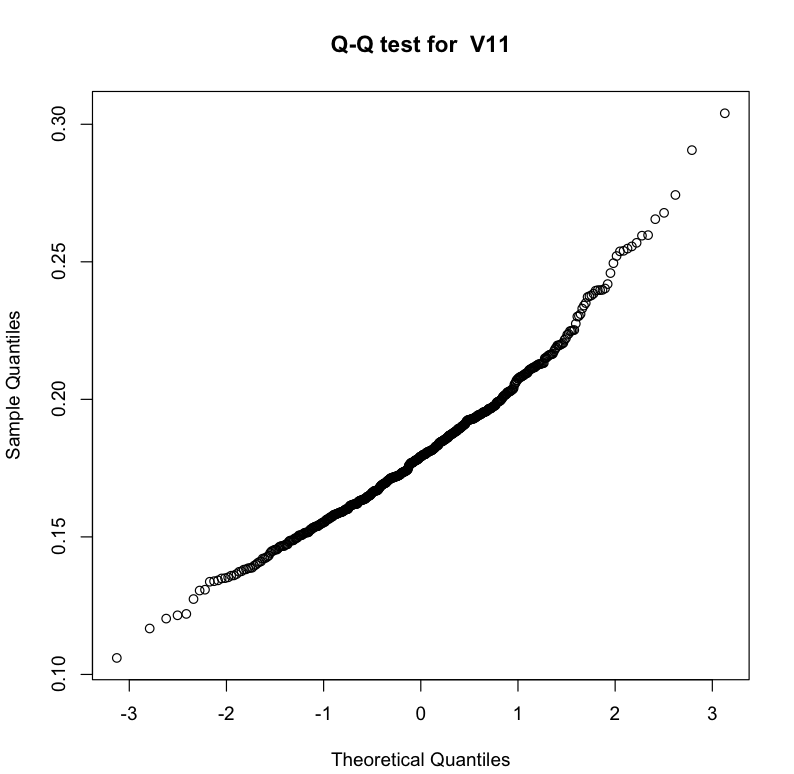
\includegraphics[scale=0.225]{pix/q_v11}
\par\end{centering}}
\end{center}
\end{figure}

\begin{figure}[H]
\begin{center}
\subfloat[]{\begin{centering}
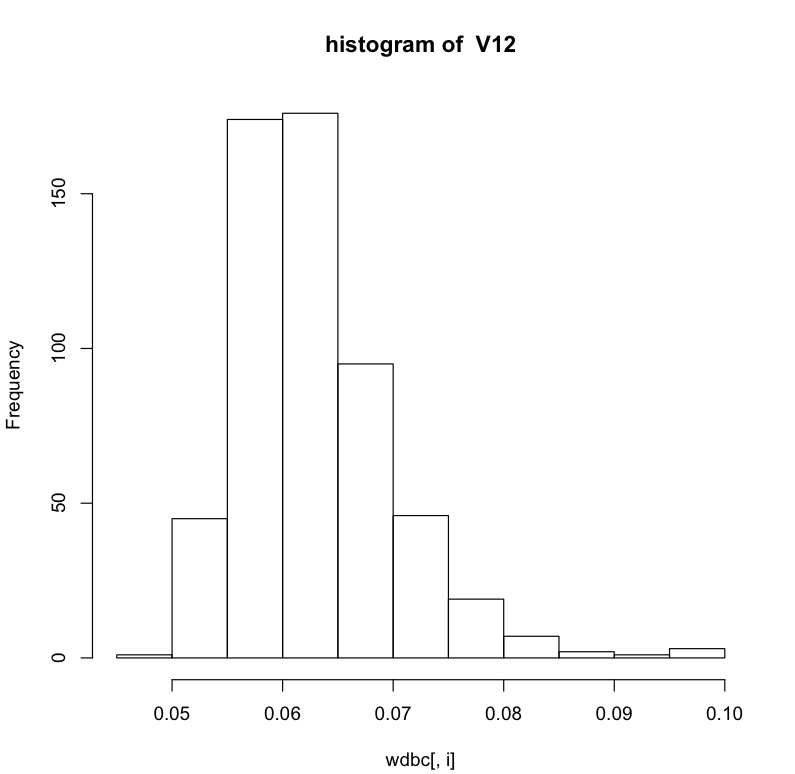
\includegraphics[scale=0.225]{pix/h_v12}
\par\end{centering}}
\quad{}
\subfloat[]{\begin{centering}
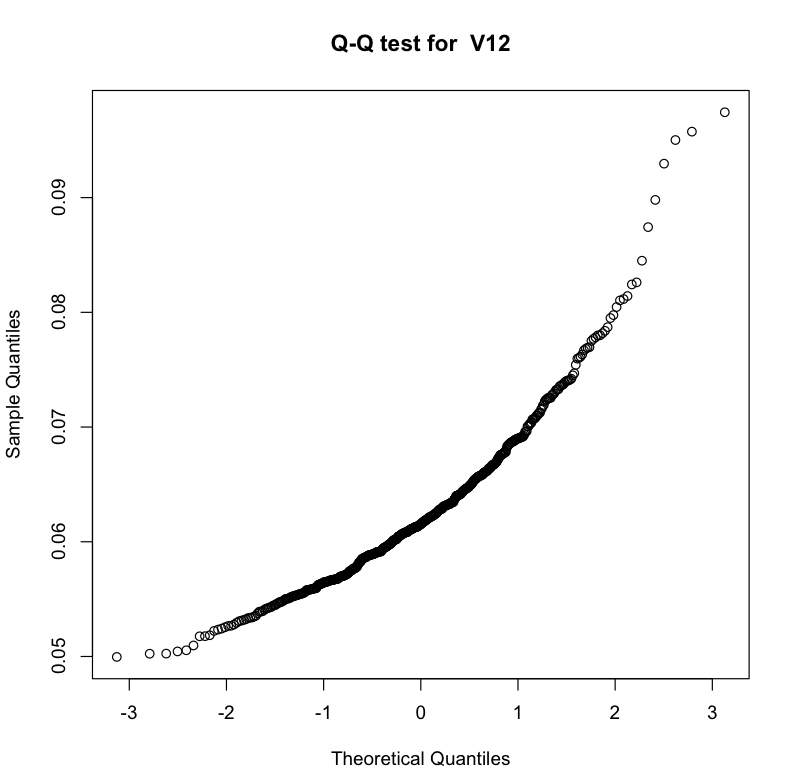
\includegraphics[scale=0.225]{pix/q_v12}
\par\end{centering}}
\quad{}
\subfloat[]{\begin{centering}
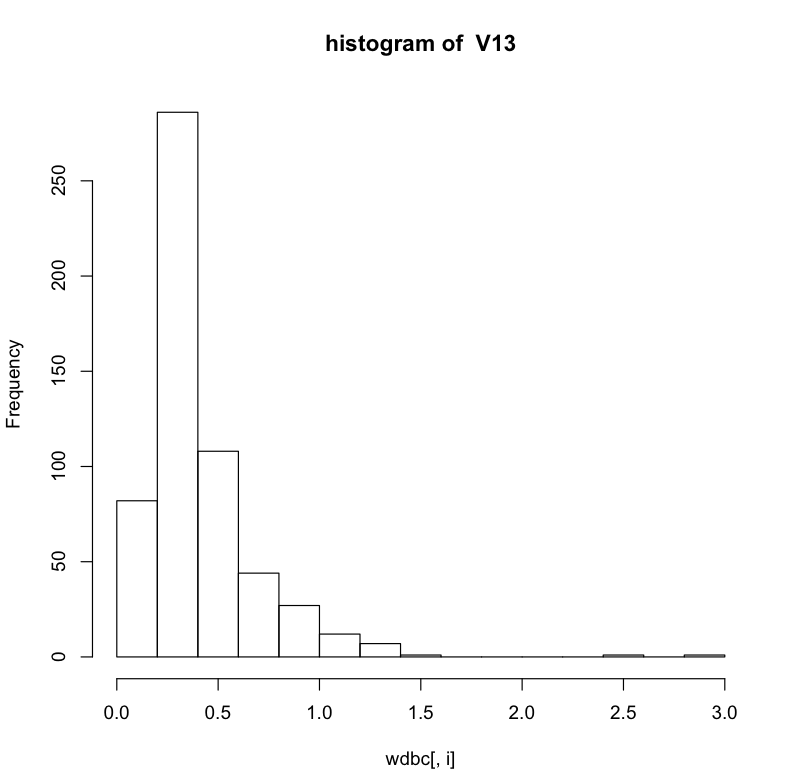
\includegraphics[scale=0.225]{pix/h_v13}
\par\end{centering}}
\quad{}
\subfloat[]{\begin{centering}
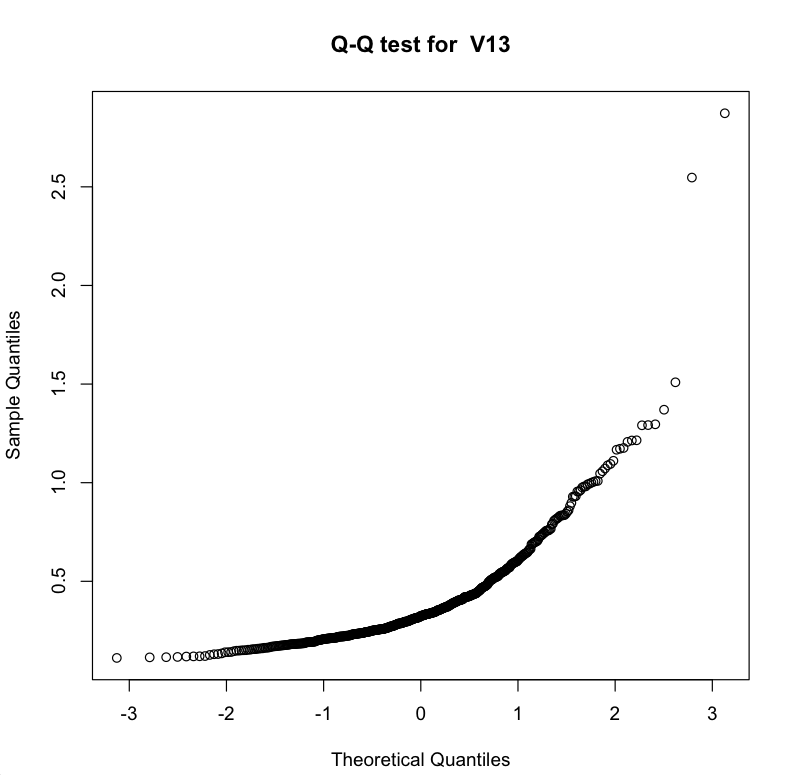
\includegraphics[scale=0.225]{pix/q_v13}
\par\end{centering}}
\quad{}
\subfloat[]{\begin{centering}
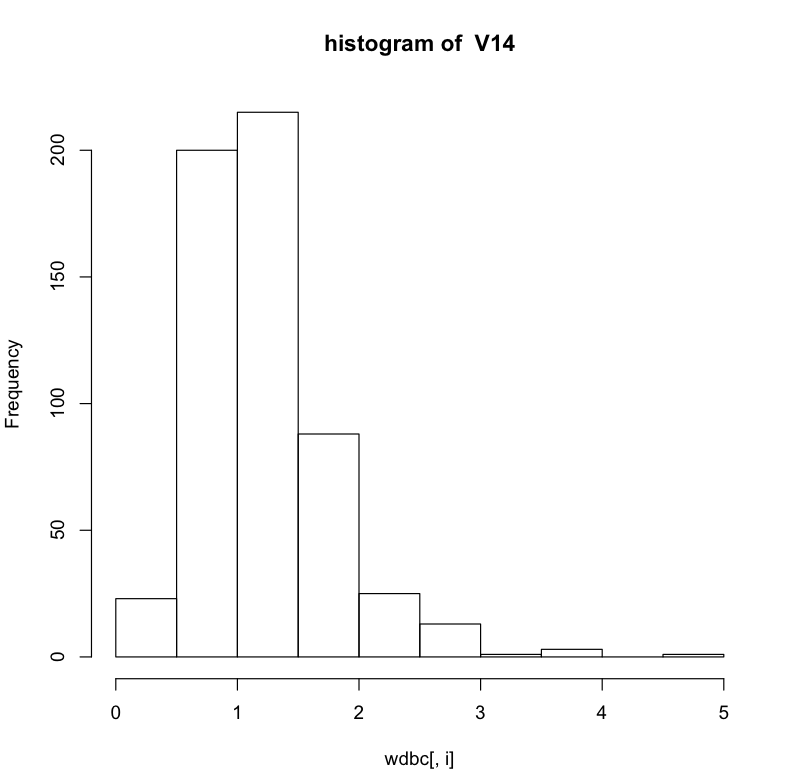
\includegraphics[scale=0.225]{pix/h_v14}
\par\end{centering}}
\quad{}
\subfloat[]{\begin{centering}
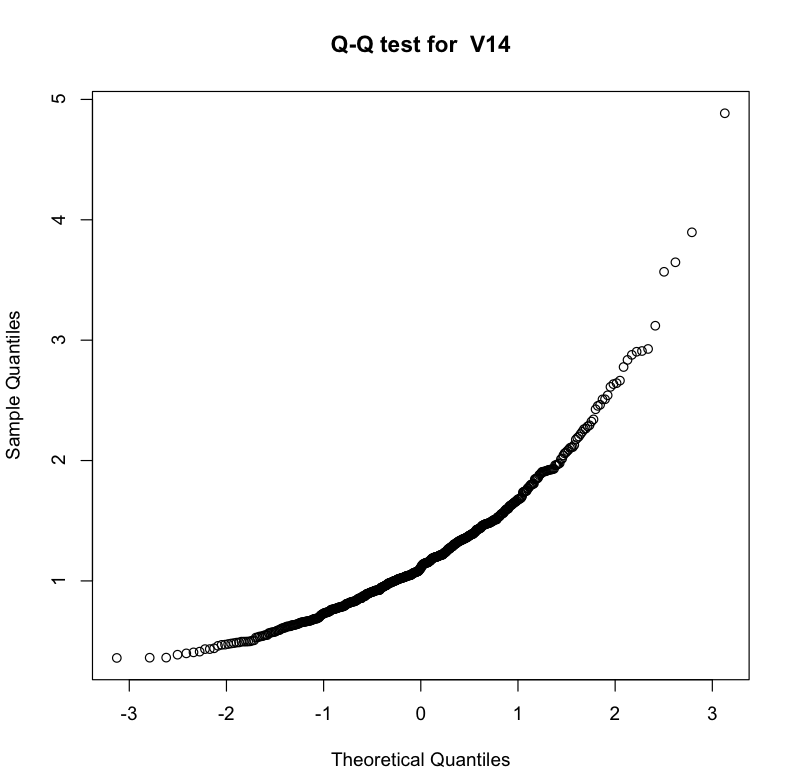
\includegraphics[scale=0.225]{pix/q_v14}
\par\end{centering}}
\end{center}
\end{figure}

\begin{figure}[H]
\begin{center}
\subfloat[]{\begin{centering}
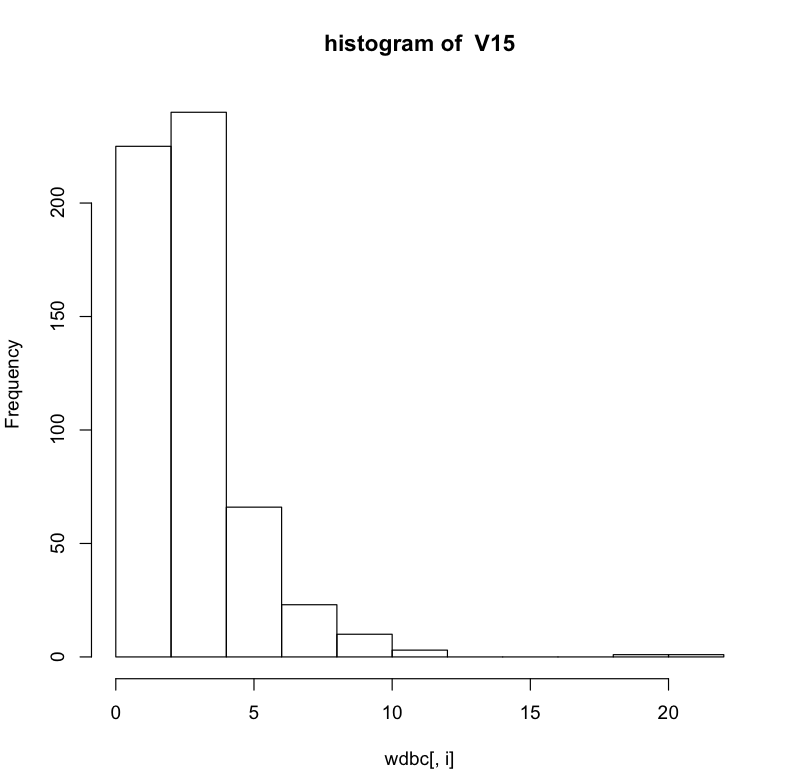
\includegraphics[scale=0.225]{pix/h_v15}
\par\end{centering}}
\quad{}
\subfloat[]{\begin{centering}
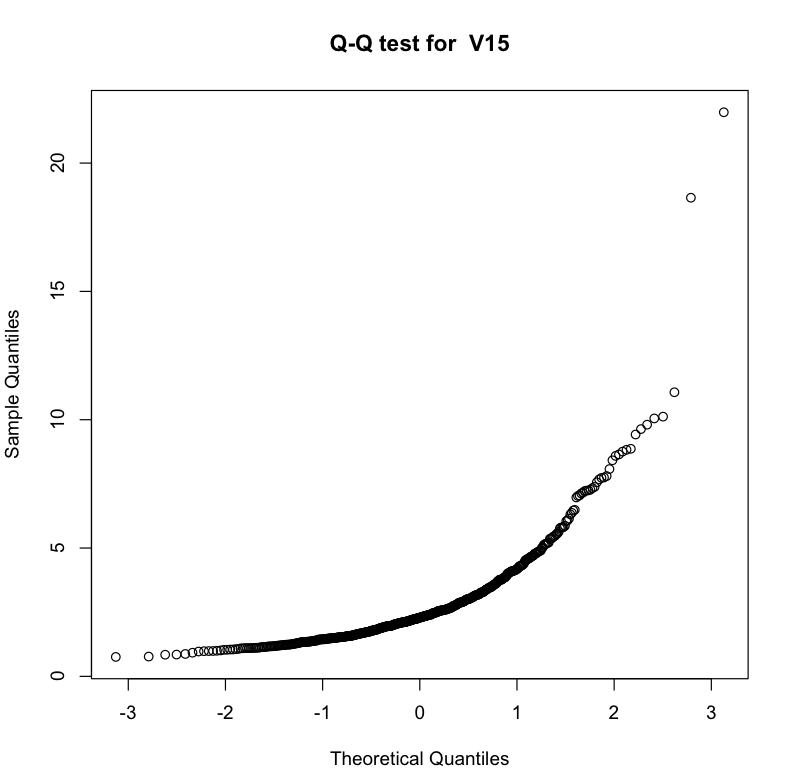
\includegraphics[scale=0.225]{pix/q_v15}
\par\end{centering}}
\quad{}
\subfloat[]{\begin{centering}
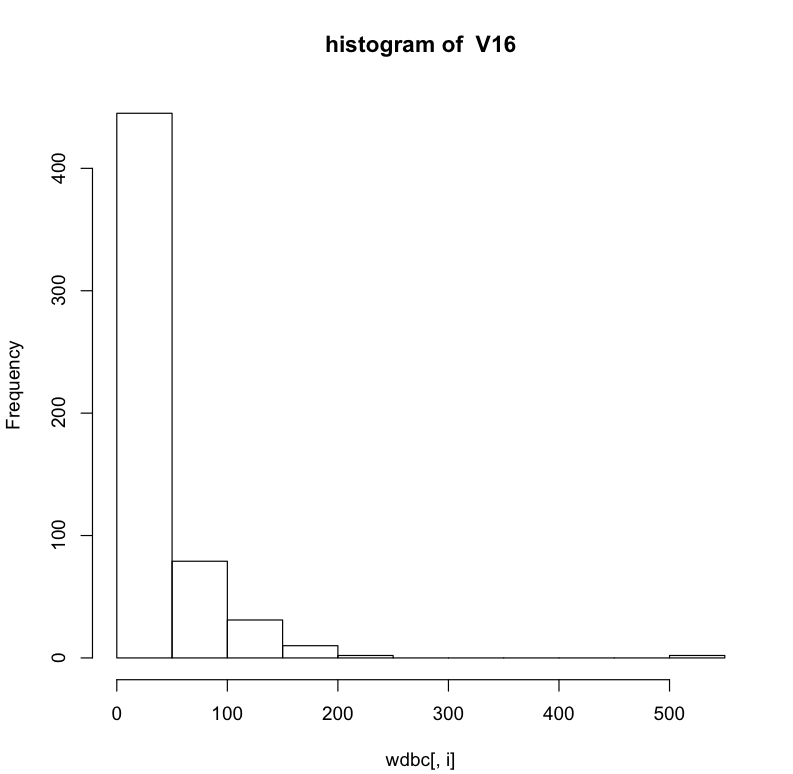
\includegraphics[scale=0.225]{pix/h_v16}
\par\end{centering}}
\quad{}
\subfloat[]{\begin{centering}
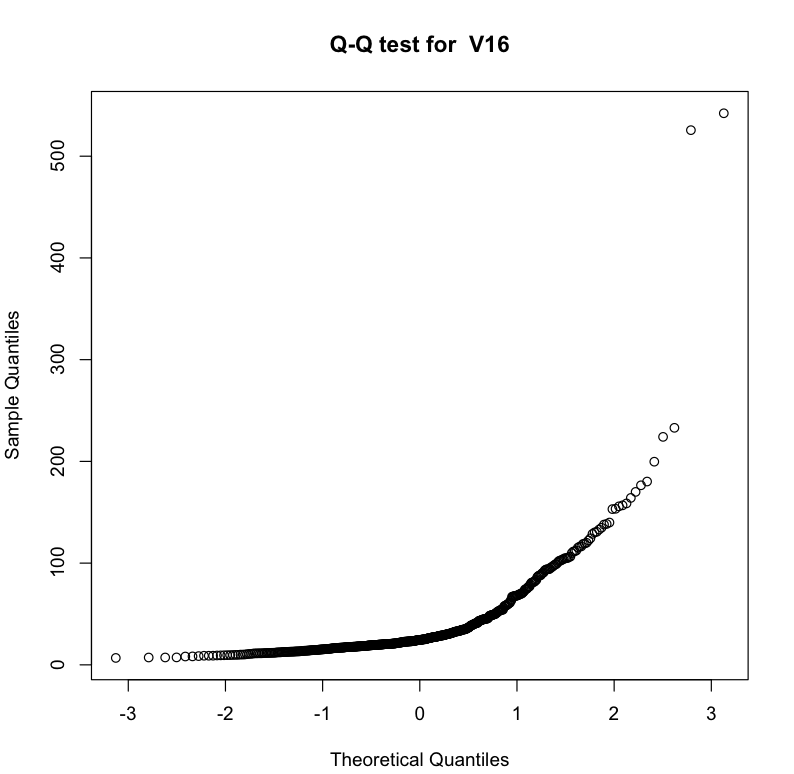
\includegraphics[scale=0.225]{pix/q_v16}
\par\end{centering}}
\quad{}
\subfloat[]{\begin{centering}
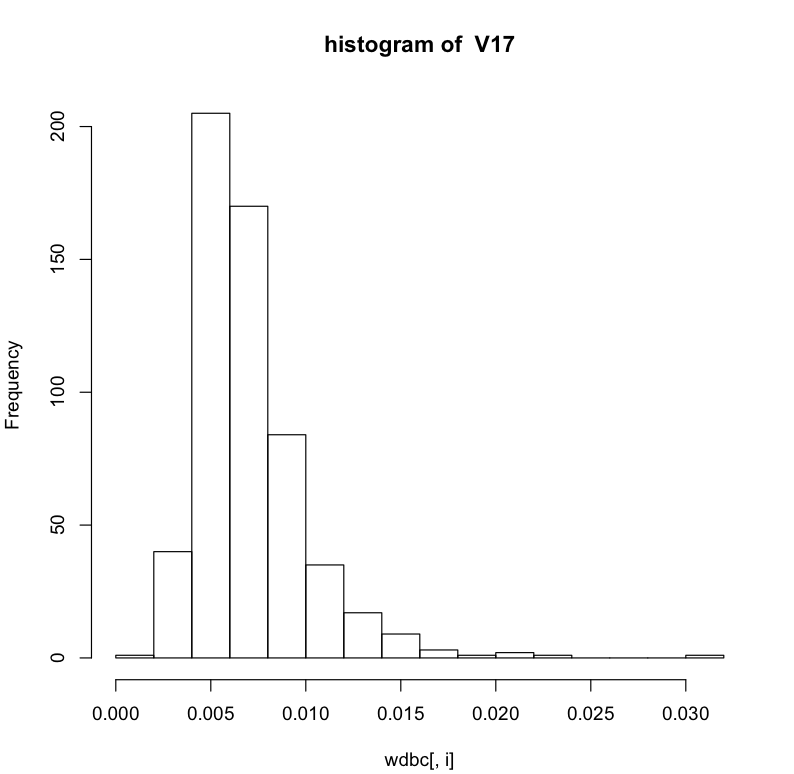
\includegraphics[scale=0.225]{pix/h_v17}
\par\end{centering}}
\quad{}
\subfloat[]{\begin{centering}
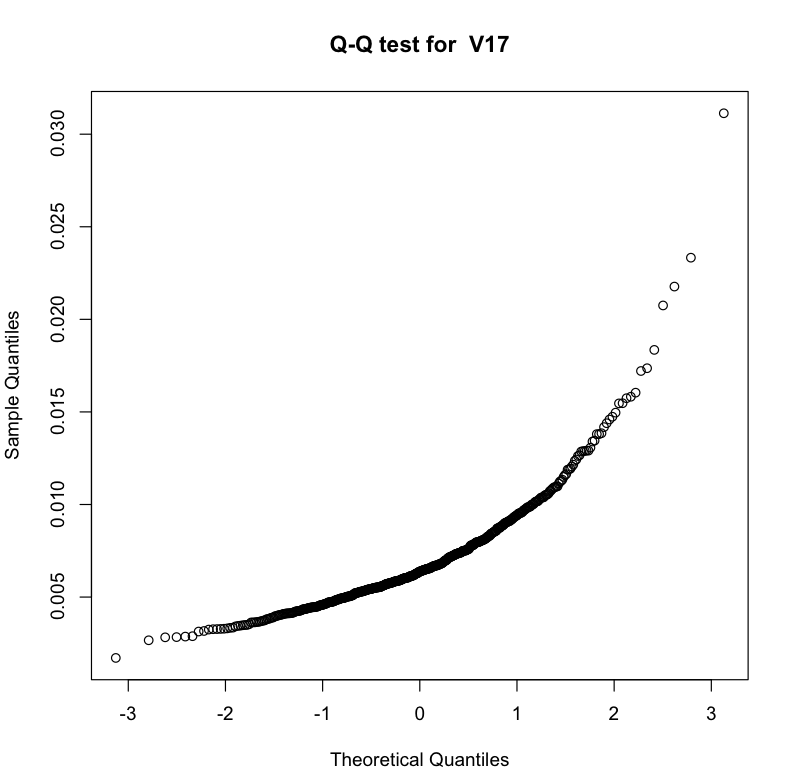
\includegraphics[scale=0.225]{pix/q_v17}
\par\end{centering}}
\end{center}
\end{figure}

\begin{figure}[H]
\begin{center}
\subfloat[]{\begin{centering}
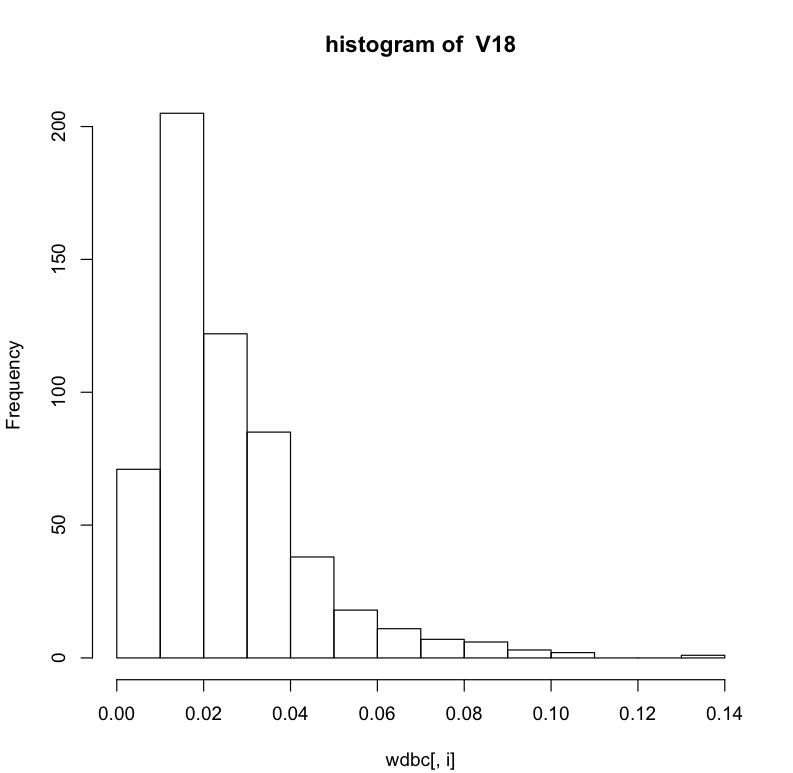
\includegraphics[scale=0.225]{pix/h_v18}
\par\end{centering}}
\quad{}
\subfloat[]{\begin{centering}
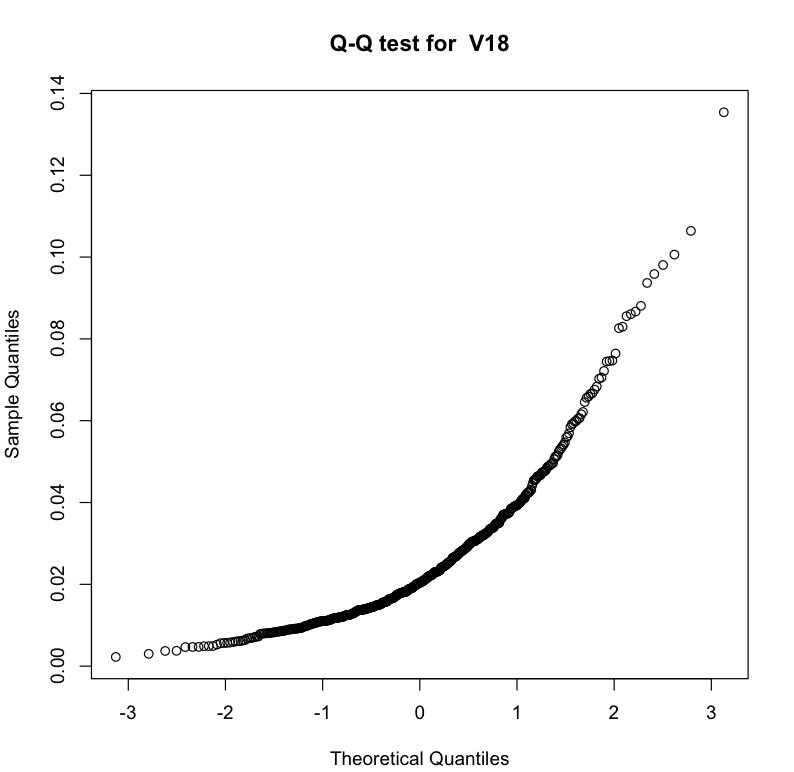
\includegraphics[scale=0.225]{pix/q_v18}
\par\end{centering}}
\quad{}
\subfloat[]{\begin{centering}
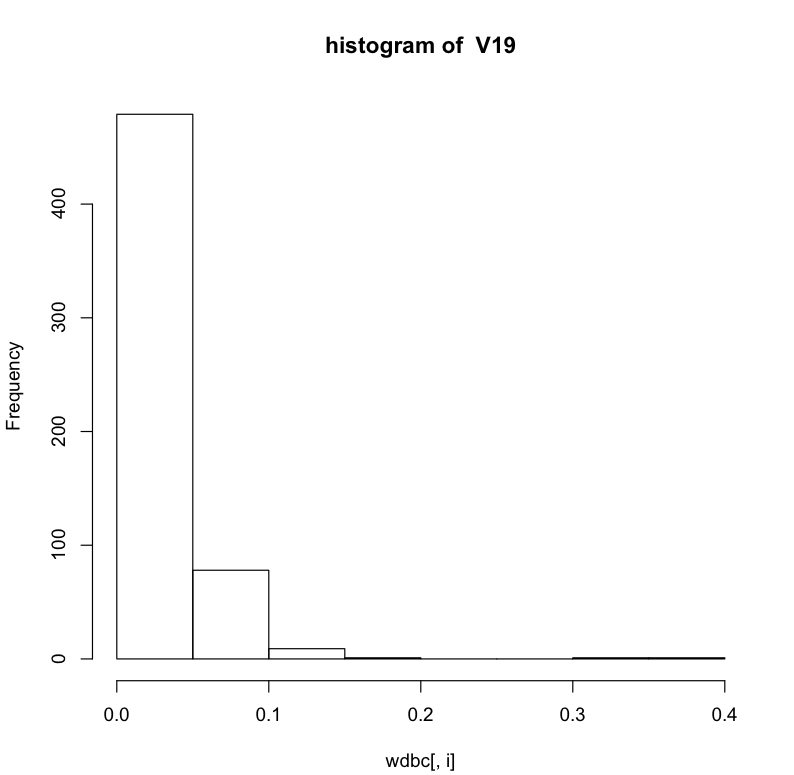
\includegraphics[scale=0.225]{pix/h_v19}
\par\end{centering}}
\quad{}
\subfloat[]{\begin{centering}
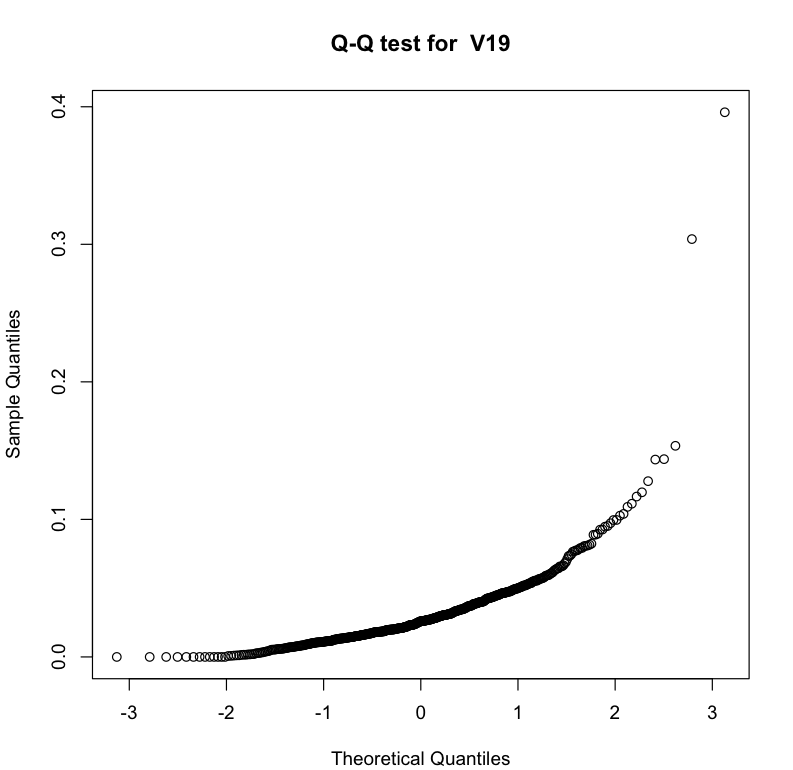
\includegraphics[scale=0.225]{pix/q_v19}
\par\end{centering}}
\quad{}
\subfloat[]{\begin{centering}
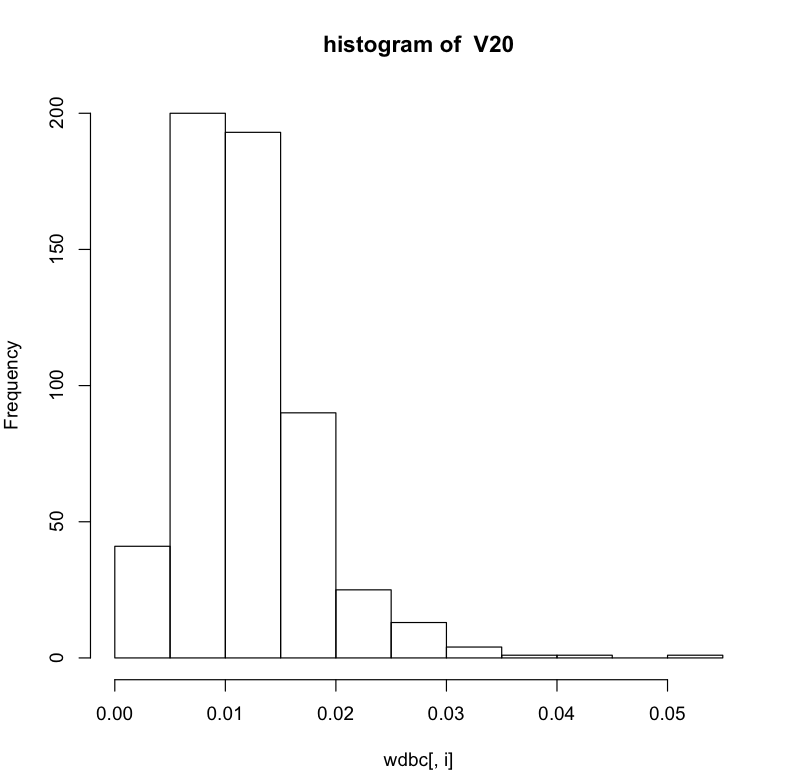
\includegraphics[scale=0.225]{pix/h_v20}
\par\end{centering}}
\quad{}
\subfloat[]{\begin{centering}
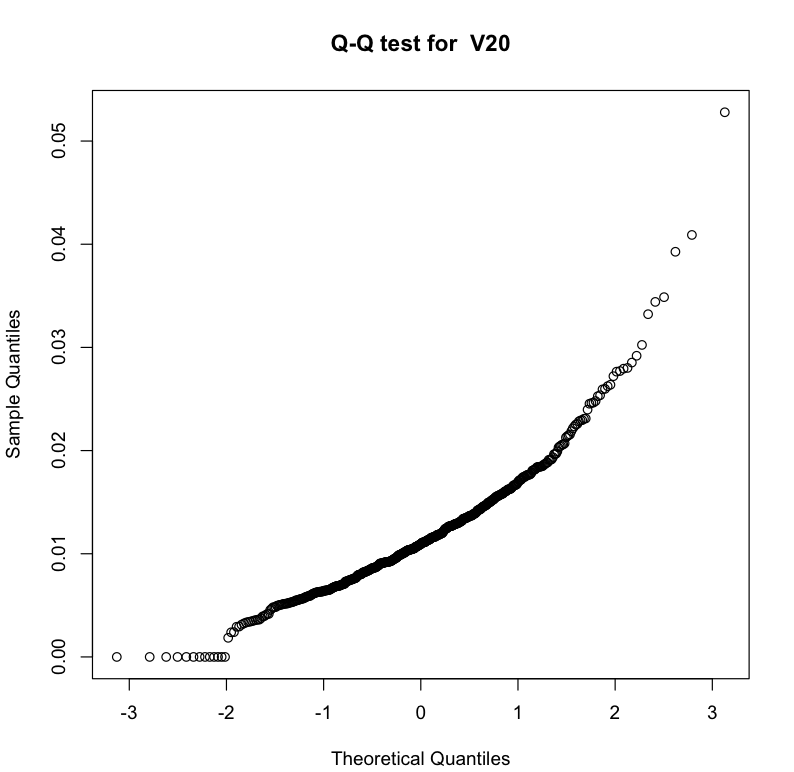
\includegraphics[scale=0.225]{pix/q_v20}
\par\end{centering}}
\end{center}
\end{figure}

\begin{figure}[H]
\begin{center}
\subfloat[]{\begin{centering}
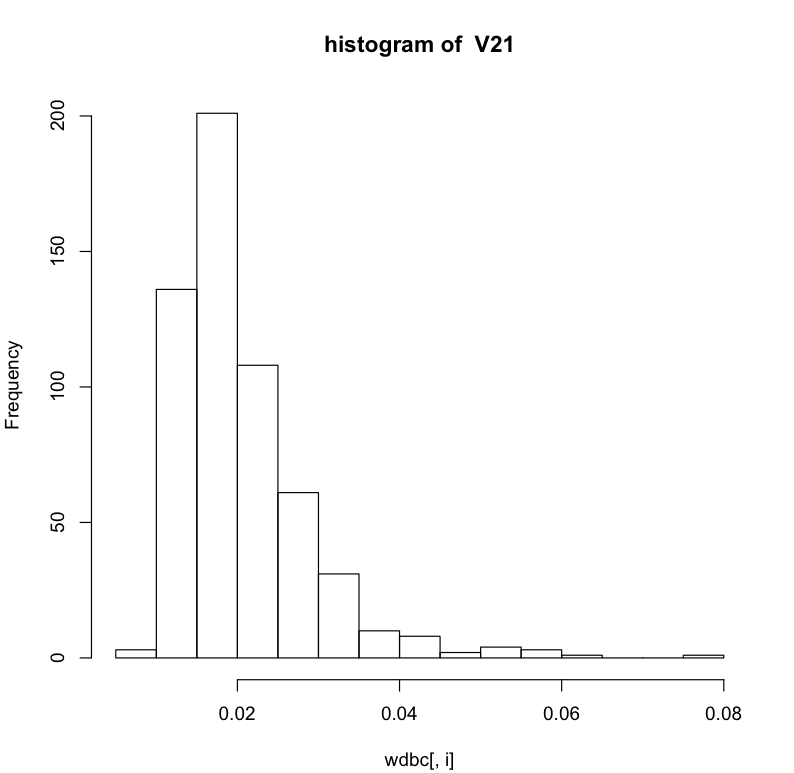
\includegraphics[scale=0.225]{pix/h_v21}
\par\end{centering}}
\quad{}
\subfloat[]{\begin{centering}
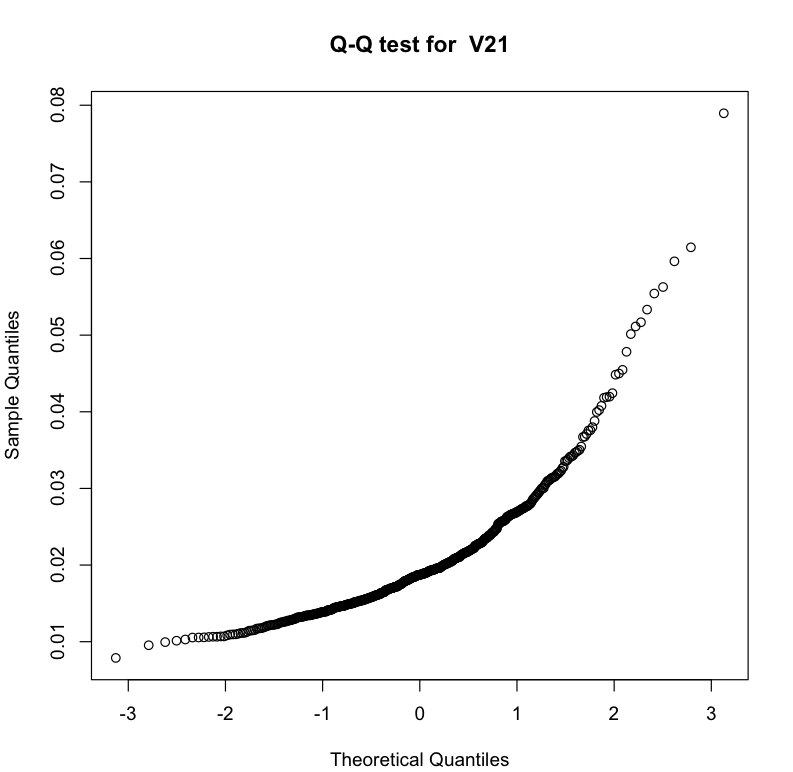
\includegraphics[scale=0.225]{pix/q_v21}
\par\end{centering}}
\quad{}
\subfloat[]{\begin{centering}
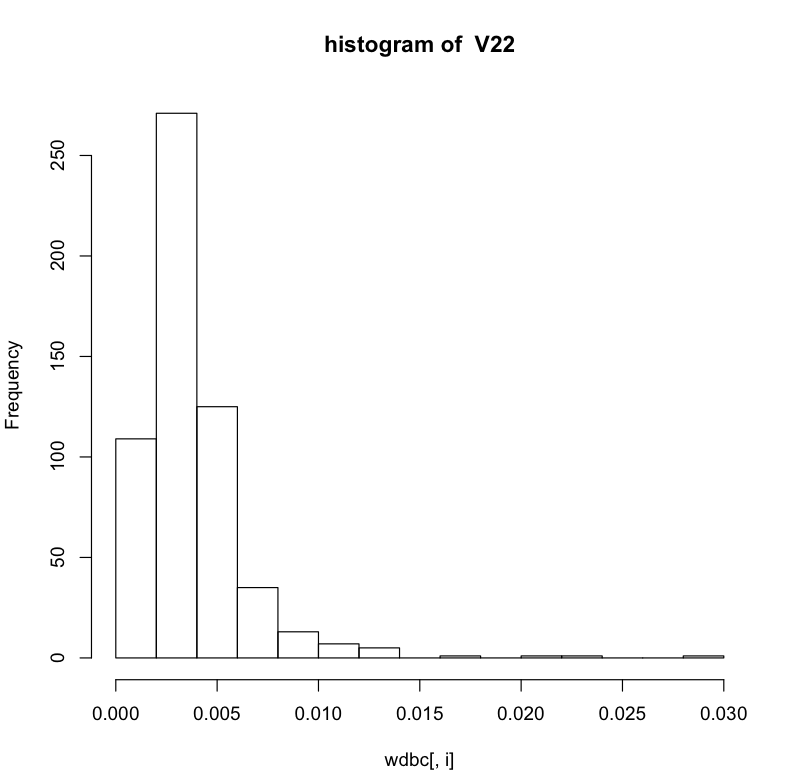
\includegraphics[scale=0.225]{pix/h_v22}
\par\end{centering}}
\quad{}
\subfloat[]{\begin{centering}
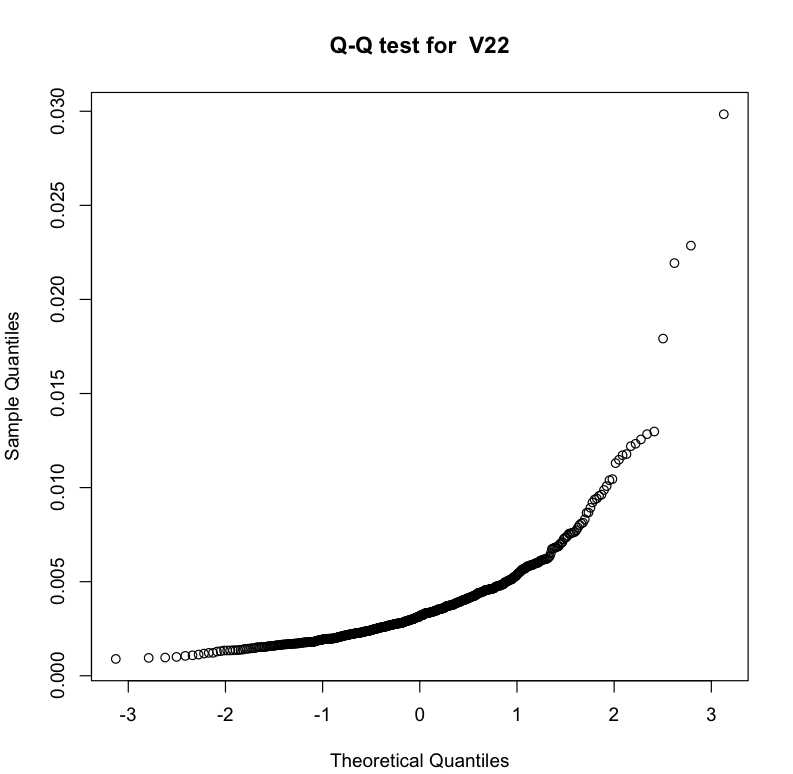
\includegraphics[scale=0.225]{pix/q_v22}
\par\end{centering}}
\quad{}
\subfloat[]{\begin{centering}
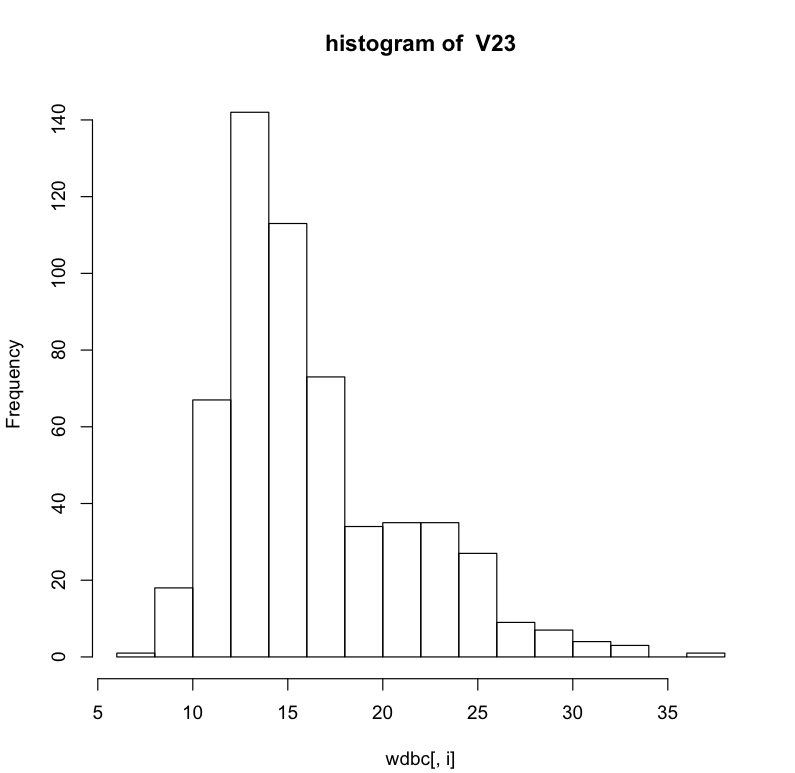
\includegraphics[scale=0.225]{pix/h_v23}
\par\end{centering}}
\quad{}
\subfloat[]{\begin{centering}
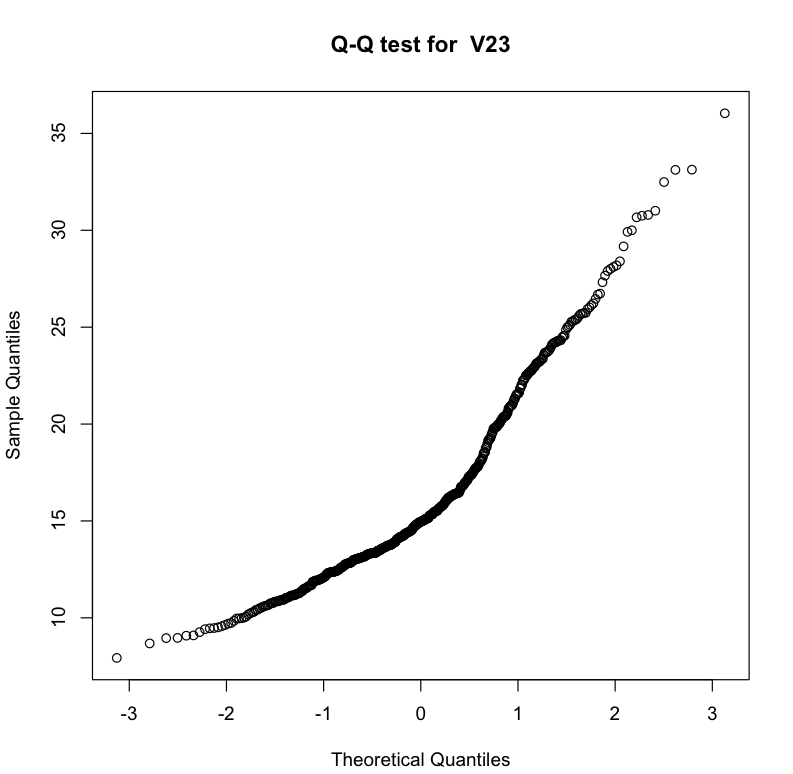
\includegraphics[scale=0.225]{pix/q_v23}
\par\end{centering}}
\end{center}
\end{figure}

\begin{figure}[H]
\begin{center}
\subfloat[]{\begin{centering}
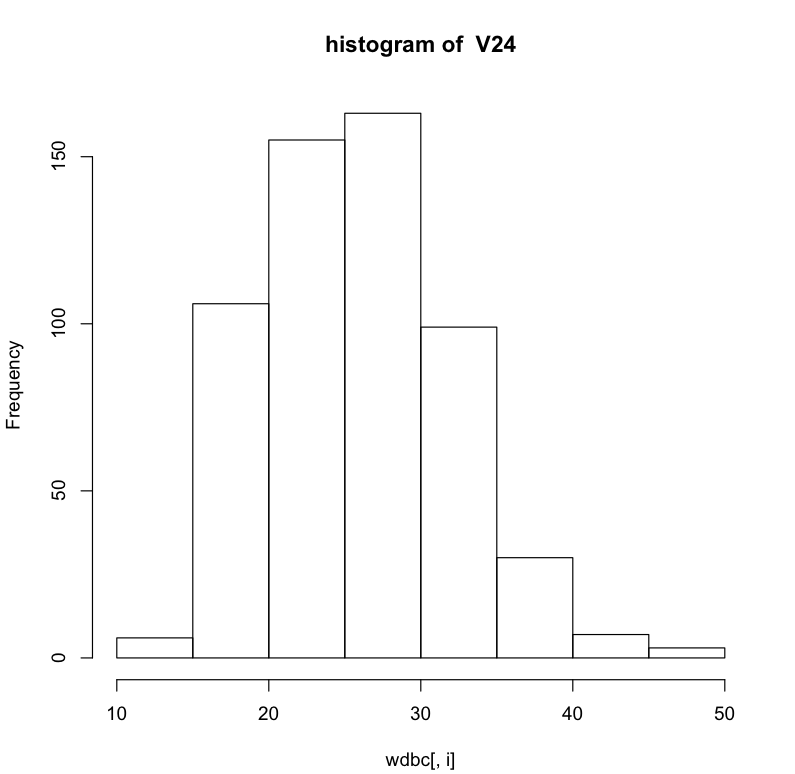
\includegraphics[scale=0.225]{pix/h_v24}
\par\end{centering}}
\quad{}
\subfloat[]{\begin{centering}
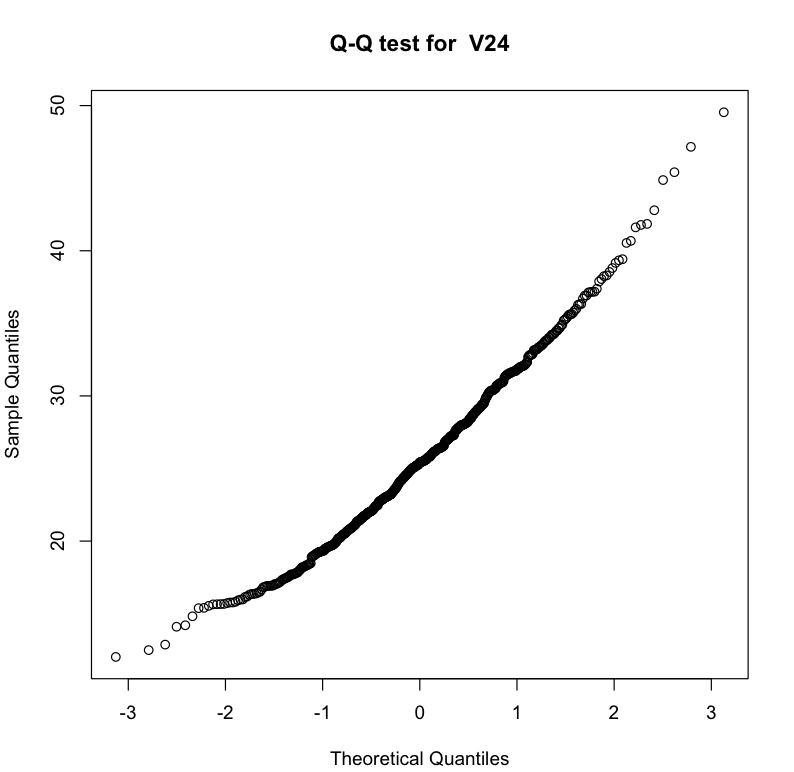
\includegraphics[scale=0.225]{pix/q_v24}
\par\end{centering}}
\quad{}
\subfloat[]{\begin{centering}
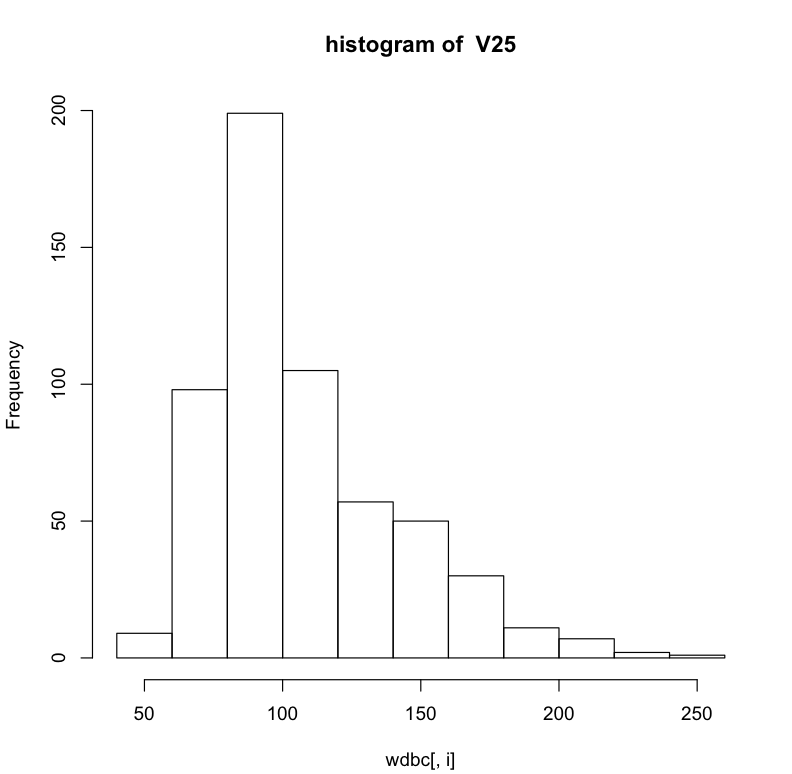
\includegraphics[scale=0.225]{pix/h_v25}
\par\end{centering}}
\quad{}
\subfloat[]{\begin{centering}
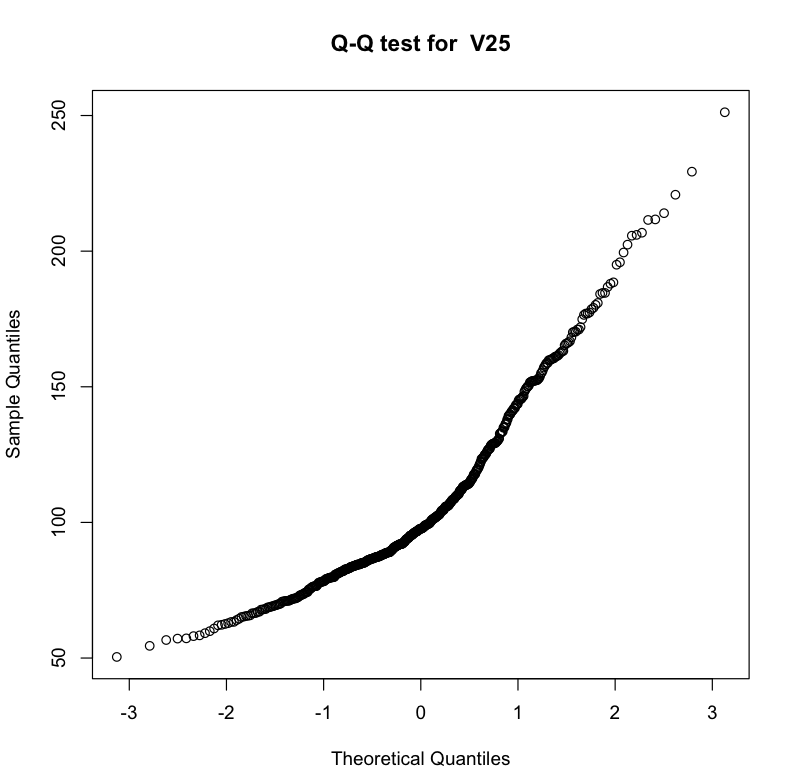
\includegraphics[scale=0.225]{pix/q_v25}
\par\end{centering}}
\quad{}
\subfloat[]{\begin{centering}
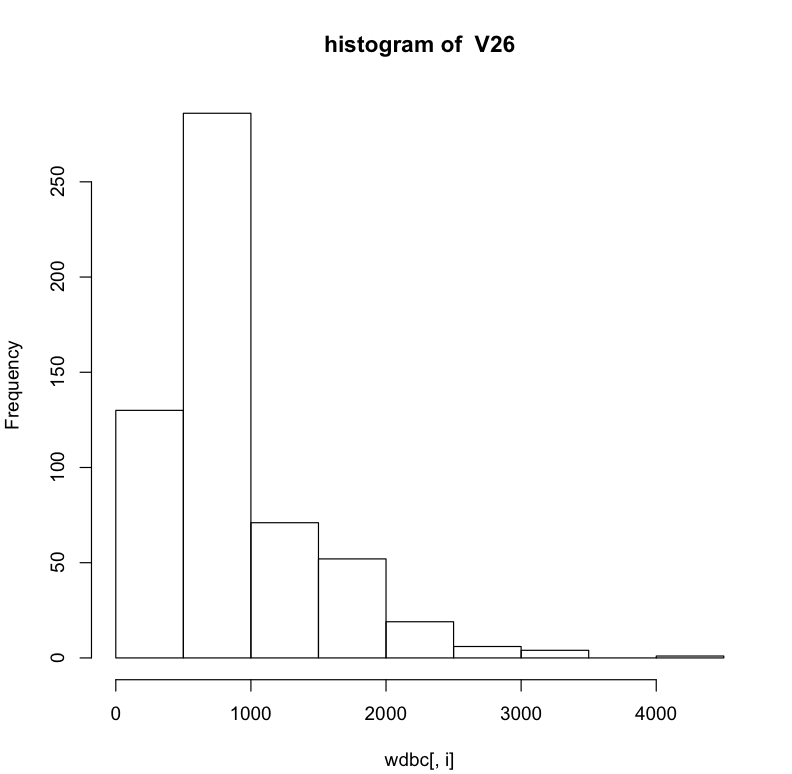
\includegraphics[scale=0.225]{pix/h_v26}
\par\end{centering}}
\quad{}
\subfloat[]{\begin{centering}
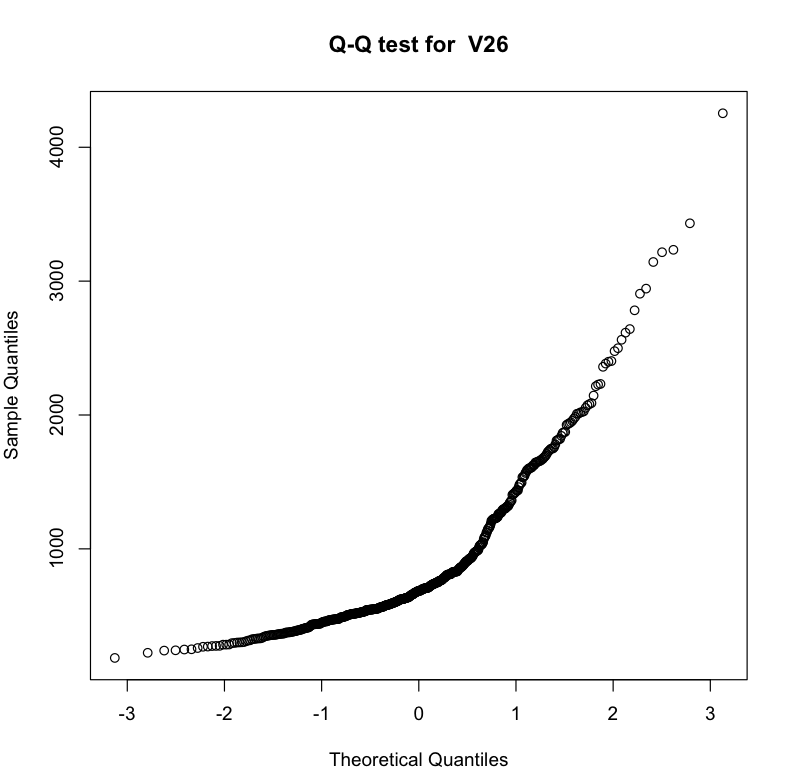
\includegraphics[scale=0.225]{pix/q_v26}
\par\end{centering}}
\end{center}
\end{figure}

\begin{figure}[H]
\begin{center}
\subfloat[]{\begin{centering}
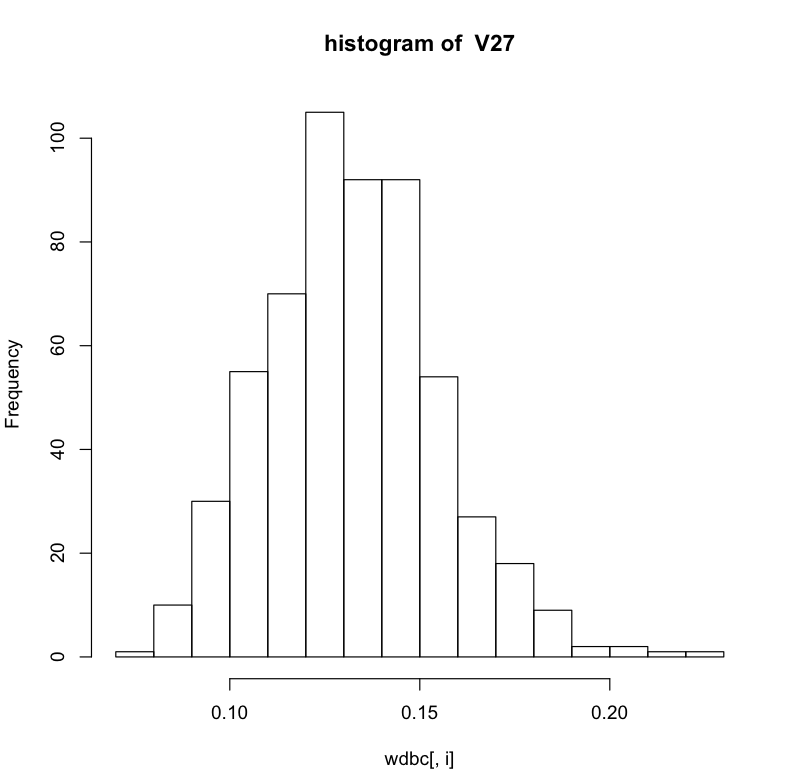
\includegraphics[scale=0.225]{pix/h_v27}
\par\end{centering}}
\quad{}
\subfloat[]{\begin{centering}
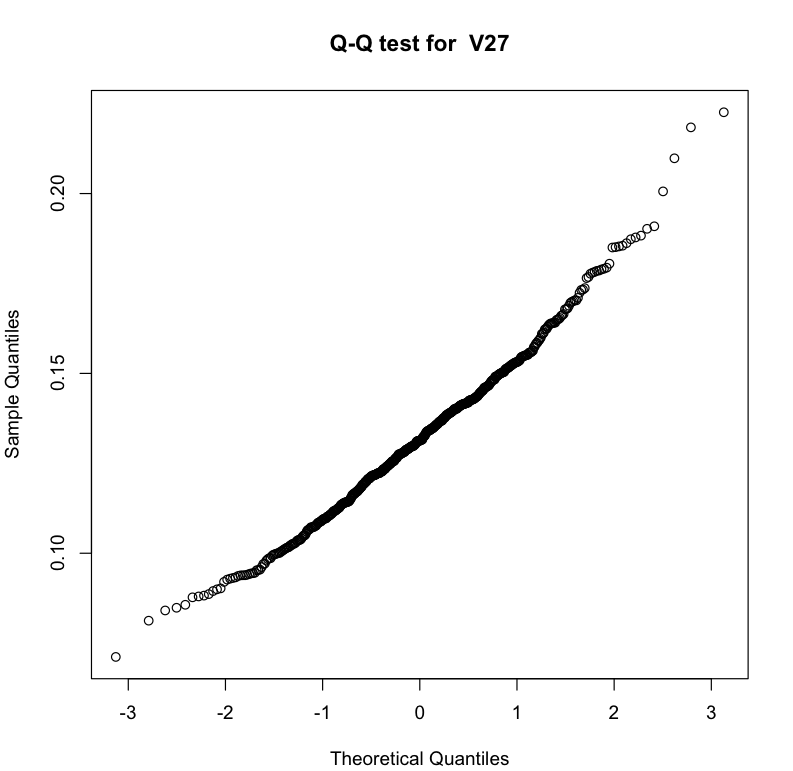
\includegraphics[scale=0.225]{pix/q_v27}
\par\end{centering}}
\quad{}
\subfloat[]{\begin{centering}
\includegraphics[scale=0.225]{pix/h_v28}
\par\end{centering}}
\quad{}
\subfloat[]{\begin{centering}
\includegraphics[scale=0.225]{pix/q_v28}
\par\end{centering}}
\quad{}
\subfloat[]{\begin{centering}
\includegraphics[scale=0.225]{pix/h_v29}
\par\end{centering}}
\quad{}
\subfloat[]{\begin{centering}
\includegraphics[scale=0.225]{pix/q_v29}
\par\end{centering}}
\end{center}
\end{figure}

\begin{figure}[H]
\begin{center}
\subfloat[]{\begin{centering}
\includegraphics[scale=0.225]{pix/h_v30}
\par\end{centering}}
\quad{}
\subfloat[]{\begin{centering}
\includegraphics[scale=0.225]{pix/q_v30}
\par\end{centering}}
\quad{}
\subfloat[]{\begin{centering}
\includegraphics[scale=0.225]{pix/h_v31}
\par\end{centering}}
\quad{}
\subfloat[]{\begin{centering}
\includegraphics[scale=0.225]{pix/q_v31}
\par\end{centering}}
\quad{}
\subfloat[]{\begin{centering}
\includegraphics[scale=0.225]{pix/h_v32}
\par\end{centering}}
\quad{}
\subfloat[]{\begin{centering}
\includegraphics[scale=0.225]{pix/q_v32}
\par\end{centering}}
\end{center}
\end{figure}

None of the histogram plots display strongly normal distributions, and the qq-plots also support the 
results of the Shapiro-Wilk test. The data in wdbc.data are not normally distributed. 

\item After splitting wdbc.data into 70\% training and 30\% test 
      data, compare the test accuracies of naive Bayes, treating
      the quantitative variables as 
  \begin{enumerate}
    \item normally distributed variables

          The accuracy for \verb|naiveBayes()| was approximately 95.3\%

    \item categorical variables with 4 levels. 

          The accuracy for \verb|naiveBayes()| was approximately 95.3 \%
  \end{enumerate}

\item Use 10-fold cross validation to estimate the accuracy of naive Bayes on wdbc.data, 
treating the quantitative variables as 

  \begin{enumerate}
    \item mormally distributed variables

          The accuracy using 10-fold cross validation was $\approx$ 93.5 \%

    \item categorical variables with $L$ levels, L = 2, 3, ... , 10.

          Below is a plot of the average error using 10-fold cross validation for the data evaluated as 
          categorical variables at each level $L$. 
          
          \begin{center}
          \includegraphics[scale=0.35]{pix/err_k10_cat}
          \end{center}

  \end{enumerate}

Which value of $L$ produces the highest accuracy? 

The smallest error for 10-fold cross validation occured when using $L = 6$
with an accuracy of approximately 95.4\%.

\item Investigate the effect of the Laplace smoothing argument in the naiveBayes function. 
What appears to be the optimal value for this argument? 

The laplace smoothing argument is a way for the algorithm to compute probabilities for anomalous data. 
That is, when a value is absent or outside of the algorithm's parameters, some method is needed for 
dealing with the missing information. Using \verb|naiveBayes()| without an entry for laplace smoothing is 
the same as calling \verb|naiveBayes( ... , laplace = 0, ...)|. 

On the wdbc.data set, the Laplace smoothing argument had no effect whatsoever. This is 
because all of the quantitative variables have real values and the one column of 
categorical variables has all entries defined. This is not so for the houseVotes84 data set. 
In this case, there are multiple entries for each vote column that have no values (entered as NA). 

The effect of the Laplace smoothing appears to be problem-specific in this case. Whether from the size of 
the data set or from the distribution of the data, each value assigned to the laplace argument affects the 
overall error rate significantly, but the manner of affecting, whether for better or worse changes 
based upon the random sample (of the same size each time) that is taken. 

Thus the error rate and the laplace value are plotted for two different samples of the same size below. 
The significance of the value of laplace is undoubtable, but it varies so greatly from case to case that 
there is no useful information to be gained from a comparison of values. 

\begin{center}
\includegraphics[scale=0.35]{pix/err_1}

\includegraphics[scale=0.35]{pix/err_2}
\end{center}

The overall trend from these two cases is for the error to increase in an oscillating way from values of 
laplace of 0 to around 2500 before reaching a maximum. However, the behaviour of the errors is so varied 
between laplace = 0 and laplace = 100 as to give no useful information except for the fact that the 
errors are overall increasing. 

To see if there is an overarching order in the different effects which the two specific cases did not 
catch, a 10-fold cross-validation was used to compute error for each value of laplace as well. 
The errors for each of these computations was stored and averaged to give the plot below. 

\begin{center}
\includegraphics[scale=0.35]{pix/10fold_cv}
\end{center}

However, the actual values of each of the 10 versions is also shown below with the specific fold 
highligthed in red to show the variation in values. 

\begin{figure}[H]
\begin{center}
\subfloat[Fold 1]{\begin{centering}
\includegraphics[scale=0.225]{pix/f1}
\par\end{centering}}
\quad{}
\subfloat[Fold 2]{\begin{centering}
\includegraphics[scale=0.225]{pix/f2}
\par\end{centering}}
\quad{}
\subfloat[Fold 3]{\begin{centering}
\includegraphics[scale=0.225]{pix/f3}
\par\end{centering}}
\quad{}
\subfloat[Fold 4]{\begin{centering}
\includegraphics[scale=0.225]{pix/f4}
\par\end{centering}}
\quad{}
\subfloat[Fold 5]{\begin{centering}
\includegraphics[scale=0.225]{pix/f5}
\par\end{centering}}
\quad{}
\subfloat[Fold 6]{\begin{centering}
\includegraphics[scale=0.225]{pix/f6}
\par\end{centering}}
\end{center}
\end{figure}

\begin{figure}[H]
\begin{center}
\subfloat[Fold 7]{\begin{centering}
\includegraphics[scale=0.225]{pix/f7}
\par\end{centering}}
\quad{}
\subfloat[Fold 8]{\begin{centering}
\includegraphics[scale=0.225]{pix/f8}
\par\end{centering}}
\quad{}
\subfloat[Fold 9]{\begin{centering}
\includegraphics[scale=0.225]{pix/f9}
\par\end{centering}}
\quad{}
\subfloat[Fold 10]{\begin{centering}
\includegraphics[scale=0.225]{pix/f10}
\par\end{centering}}
\end{center}
\end{figure}

Below a value of 2500 is therefore the best guess at an optimal value for the laplace argument 
for this problem.

Note that for values of laplace $\le$ 1, the variation in error is so great as to obscure any pattern whatsoever. 

\begin{figure}[H]
\begin{center}
\subfloat[Fold 1]{\begin{centering}
\includegraphics[scale=0.225]{pix/f11}
\par\end{centering}}
\quad{}
\subfloat[Fold 2]{\begin{centering}
\includegraphics[scale=0.225]{pix/f12}
\par\end{centering}}
\quad{}
\subfloat[Fold 3]{\begin{centering}
\includegraphics[scale=0.225]{pix/f13}
\par\end{centering}}
\quad{}
\subfloat[Fold 4]{\begin{centering}
\includegraphics[scale=0.225]{pix/f14}
\par\end{centering}}
\quad{}
\subfloat[Fold 5]{\begin{centering}
\includegraphics[scale=0.225]{pix/f15}
\par\end{centering}}
\quad{}
\subfloat[Fold 6]{\begin{centering}
\includegraphics[scale=0.225]{pix/f16}
\par\end{centering}}
\end{center}
\end{figure}

\begin{figure}[H]
\begin{center}
\subfloat[Fold 7]{\begin{centering}
\includegraphics[scale=0.225]{pix/f17}
\par\end{centering}}
\quad{}
\subfloat[Fold 8]{\begin{centering}
\includegraphics[scale=0.225]{pix/f18}
\par\end{centering}}
\quad{}
\subfloat[Fold 9]{\begin{centering}
\includegraphics[scale=0.225]{pix/f19}
\par\end{centering}}
\quad{}
\subfloat[Fold 10]{\begin{centering}
\includegraphics[scale=0.225]{pix/f101}
\par\end{centering}}
\end{center}
\end{figure}
\end{enumerate}

\begin{center}
\includegraphics[scale=0.35]{pix/kf_v}
\end{center}

\begin{Verbatim}
# Data Mining hw 8
library(e1071)
data(houseVotes84, package='pmml')

#1. For the following problems, consult the HouseVotes84 
#   data set. 

##a. What is the probability that a randomly selected 
##   representative is a Democrat? 
  print(sum(houseVotes84$Class == 'democrat')/nrow(houseVotes84))
  # probability is 61% it wil be a Democrat

  # alt way: 
  print(table(houseVotes84$Class) / sum(table(houseVotes84$Class)))

##b. Given that a representative is a Republican, what 
##   is the probability that he or she voted for water 
##   project cost sharing? 

  repwater <- naiveBayes(V2~Class, houseVotes84)

  ##Verify by hand computation of Bayes formula: 
  rep <- (houseVotes84$Class == 'republican') * 1
  dem <- (houseVotes84$Class == 'democrat') * 1

  idx <- 1 - (is.na(houseVotes84$V2) * 1) 
  v2 <- houseVotes84$V2[complete.cases(houseVotes84$V2)]

  prob_water = sum( (v2 == 'y') * 1) / length(v2)
  prob_nwater = sum((v2 == 'n') * 1) / length(v2)
  prob_rep = sum(rep) / nrow(houseVotes84)
  prob_dem = sum(dem) / nrow(houseVotes84)
  p_w_rep = sum( (v2 == 'y') & (rep[idx == 1] > 0) ) / (sum(rep))
  p_w_dem = sum( (v2 == 'y') & (dem[idx == 1] > 0) ) / (sum(dem))

  # probability is 0.3846154 by both computations.

##c. Given that a representative voted for adoption of the 
##   budget resolution, against the physician fee freeze and 
##   for duty free exports, find the probability that he or she 
##   is a Democrat (Hint: if x is a vector, you can use 
##   rbind(x) to force R to treat it as a row vector. You can 
##   set missing values of x to NA, and naive Bayes will 
##   ignore them.)
##
##      i.e. We're checking probability that
##        Class == 'democrat' given 
##        V3 = 'y'
##        V4 = 'n'
##        V15 = 'y'

  dem3415 <- naiveBayes(Class~V3 + V4 + V15, houseVotes84)
  dvec <- rbind(rep('NA', 17))
  dvec[4] <- 'y'
  dvec[5] <- 'n'
  dvec[16] <- 'y'
  predict(dem3415, newdata = dvec, type='raw')

#2. Investigate normality of the quantitative variables in the 
#   wdbc.data data set, using Shapiro-Wilk tests, histograms, 
#   and qq-plots. 
  wdbc <- read.table('~/Dropbox/Tarleton/data_mining/hw05/wdbc.data',
                     header=F,sep=',')
  wdbc <- wdbc[,-1]
  names(wdbc)[1] <- c('diagnosis')

  for(i in 2:ncol(wdbc)){
  	name <- toString(names(wdbc)[i])
  	hist(wdbc[,i], main=paste('histogram of ',name))
  	print(paste(name, shapiro.test(wdbc[,i])$p))
  	qqnorm(wdbc[,i], main=paste('Q-Q test for ',name))
  }

#3. After splitting wdbc.data into 70% training and 30% test 
#   data, compare the test accuracies of naive Bayes, treating 
#   the quantitative variables as 

  splitset <- splitdata(wdbc, 0.7, FALSE)
  train_d <- splitset$traindata
  test_d  <- splitset$testdata
  train_i <- splitset$train

##a. normally distributed variables
  pred_diag_n <- naiveBayes(diagnosis ~., wdbc[train_i,])
  pred <- predict(pred_diag_n, wdbc[-train_i,])
  table(pred, wdbc$diagnosis[-train_i])
  err_normal = confmatrix(wdbc$diagnosis[-train_i], pred)$error

##b. categorical variables with 4 levels. 

  disc_wdbc <- wdbc
  for (j in 2:ncol(wdbc)){
    disc_wdbc[,j] <- cut(wdbc[,j], 4)
  }
  pred_diag_n <- naiveBayes(diagnosis ~., disc_wdbc[train_i,])
  pred <- predict(pred_diag_n, disc_wdbc[-train_i,])
  table(pred, disc_wdbc$diagnosis[-train_i])
  err_cat = confmatrix(disc_wdbc$diagnosis[-train_i], pred)$error

#4. Use 10-fold cross validation to estimate the accuracy of 
#   naive Bayes on wdbc.data, treating the quantitative 
#   variables as 

##a. normally distributed variables
err_k10_normal1 <- kfold_val(10, 2, wdbc, 1)$error

# 0.6616758

##b. categorical variables with L levels, L = 2, 3, ... , 10.
  nlevels = 10
  err_k10_cat <- 1:nlevels

  for(L in 2:nlevels){
    disc <- wdbc
    for(j in 2:ncol(wdbc)){
      disc[,j] <- cut(wdbc[,j], L)
    }
    err_k10_cat[L] <- kfold_val(10, 2, disc, 1)
  }
  v1 = 2:L
  plot(v1, err_k10_cat[2:L], 
      xlab='# levels', ylab='kfold error', type='p', pch=16,
      col=c('black','blue',
            'green','yellow',
            'orange','red',
            'purple','brown',
            'gray','pink')[v1])

# highest accuracy occurs when the number of levels is: 
which.min(err_k10_cat)

#5. Investigate the effect of the Laplace smoothing argument in 
#   the naiveBayes function. What appears to be the optimal value
#   for this argument? 
  splitset1 <- splitdata(houseVotes84, 0.7, FALSE)
  train_d1 <- splitset1$traindata
  test_d1  <- splitset1$testdata
  train_i1 <- splitset1$train

myl = seq(from=0,to=3,by=0.15)
len=length(myl)
k = 10

err = rep(-1, len)
k_err = rep(-1, len)
k_errs_for_plot <- matrix(, nrow=len, ncol=k)

for(i in 1:len){

   pred <- naiveBayes(Class~., houseVotes84[train_i1,], laplace=myl[i])
   err[i] <- confmatrix(
           predict(pred, houseVotes84[-train_i1,]), 
           houseVotes84$Class[-train_i1])$error

  l <- kfold_val(k, 3, houseVotes84, 1, myl[i])
  k_err[i] <- l$error
  k_errs_for_plot[i,] <- l$accuracy

}

for(i in 1:k){
plot(myl, k_errs_for_plot[,i], type='p',col='red', 
     ylab='error', main=paste('fold # ', toString(i)))
  for(j in 1:k){
  	if(j != i){
      lines(myl, k_errs_for_plot[,j], type='p',col='black')
    }
  }
}

plot(myl, as.numeric(k_err),xlab='Value for laplace smoothing',ylab='error',
      main='naiveBayes with k-fold cv and varying laplace')


\end{Verbatim}
\end{document}
